% This is "aamas2010_submissionExample.tex" July 2010
% This file should be compiled with "aamas2010.cls" July 2010
%
% This example file demonstrates the use of the 'aamas2010.cls'
% LaTeX2e document class file. It is for those submitting
% articles to AAMAS 2010 conference. This file is based on
% the sig-alternate.tex example file.
% The 'sig-alternate.cls' file of ACM will produce a similar-looking,
% albeit, 'tighter' paper resulting in, invariably, fewer pages.
% than the original style ACM style.
%
% ----------------------------------------------------------------------------------------------------------------
% This .tex file (and associated .cls ) produces:
%       1) The Permission Statement
%       2) The Conference (location) Info information
%       3) The Copyright Line with AAMAS data
%       4) NO page numbers
%
% as against the acm_proc_article-sp.cls file which
% DOES NOT produce 1) thru' 3) above.
%
% Using 'aamas2010.cls' you don't have control
% from within the source .tex file, over both the CopyrightYear
% (defaulted to 200X) and the IFAAMAS Copyright Data
% (defaulted to X-XXXXX-XX-X/XX/XX).
% These information will be overwritten by fixed AAMAS 2010 information
% in the style files - it is NOT as you are used with ACM style files.
%
% ---------------------------------------------------------------------------------------------------------------
% This .tex source is an example which *does* use
% the .bib file (from which the .bbl file % is produced).
% REMEMBER HOWEVER: After having produced the .bbl file,
% and prior to final submission, you *NEED* to 'insert'
% your .bbl file into your source .tex file so as to provide
% ONE 'self-contained' source file.
%
% This is the document class for full paper submission
\documentclass{aamas2010}

% if you are using PDF LaTex and you cannot find a way for producing
% letter, the following explicit settings may help

\pdfpagewidth=8.5truein
\pdfpageheight=11truein



% Use the postscript times font!
\usepackage{times}

% the following package is optional:
\usepackage{latexsym} 
\usepackage{amsmath}
\usepackage{amssymb}
\usepackage{subfigure}

% Load pfg package for drawing transition systems
\usepackage{xspace}
\usepackage{url}

\usepackage{tikz,pgf}
\usetikzlibrary{arrows,automata,trees,plotmarks,calc}


\usepackage{algorithm}
\usepackage{algorithmic}
%\usepackage[ruled,vlined]{algorithm2e}



% \renewcommand{\baselinestretch}{0.965}

\usepackage{comment}



%%%%%%%%%%%%%%%%%%%%%%%%%%%%%%%%%%%%%%%%%%%%%%%%%%%%%%%%%%%%%%%%%%%%%%%%
%%%%% START OF MACROS
%%%%%%%%%%%%%%%%%%%%%%%%%%%%%%%%%%%%%%%%%%%%%%%%%%%%%%%%%%%%%%%%%%%%%%%%
%%%%%%%%%%%%%%%%%%%%%%%%%%%%%%%%%%%%%%%%%%%%%%%%%%%%
% PERSONAL LaTex MACROS 
%	SEBASTAN SARDINA -- ssardina@cs.rmit.edu.au
%%%%%%%%%%%%%%%%%%%%%%%%%%%%%%%%%%%%%%%%%%%%%%%%%%%%



%%%%%%%%%%%%%%%%%%%%%%%%%%%%%%%%%%%%%%%%%%%%%%%%%%%%
% Font modes & definitions
%%%%%%%%%%%%%%%%%%%%%%%%%%%%%%%%%%%%%%%%%%%%%%%%%%%%

% conditional math environment
% \gdef\Math#1{\ifmmode #1 \else \mbox{$#1$}\fi}
\newcommand{\Math}[1]{\ensuremath{#1}}



\newcommand{\modesf}[1]{{\Math{\mathsf{#1}}}}
\newcommand{\modecal}[1]{{\Math{\mathcal{#1}}}}
\newcommand{\modeit}[1]{{\Math{\mathit{#1}}}}


\newcommand{\textmath}[1]{{\mbox{\textit{#1}}}}


%%%%%%%%%%%%%%%%%%%%%%%%%%%%%%%%%%%%%%%%%%%%%%%%%%%%
% Proper names
%%%%%%%%%%%%%%%%%%%%%%%%%%%%%%%%%%%%%%%%%%%%%%%%%%%%
\newcommand{\propername}[1]{\mbox{\small \textsf{#1}}}

\newcommand{\Golog}{\propername{Golog}}
\newcommand{\GologSpeak}{\propername{GologSpeak}}
\newcommand{\DGolog}{\propername{DGolog}}
\newcommand{\sGolog}{\propername{sGolog}}
\newcommand{\ConGolog}{\propername{ConGolog}}
\newcommand{\IndiGolog}{\propername{IndiGolog}}
\newcommand{\LeGolog}{\propername{LeGolog}}
\newcommand{\DTGolog}{\propername{DTGolog}}
\newcommand{\Prolog}{\propername{Prolog}}
\newcommand{\AgentSpeak}{\propername{AgentSpeak}}
\newcommand{\JASON}{\propername{Jason}}
\newcommand{\CANMINUS}{\propername{\CAN$^{\A}$}}
\newcommand{\CANMINUST}{\propernametiny{Can$^{\cal C}$}}
\newcommand{\CAN}{\propername{CAN}}
\newcommand{\CANT}{\propernametiny{Can}}
\newcommand{\CANPLAN}{\propername{CANPlan}}
\newcommand{\CANPLANT}{\propernametiny{CanPlan}}
\newcommand{\CANPLANII}{\propername{CanPlan2}}
\newcommand{\CANPLANOR}{\propername{Can(Plan)}}
\newcommand{\CANGOAL}{\propername{CanGoal}}
\newcommand{\JACK}{\propername{JACK}}
\newcommand{\weka}{\propername{weka}}
\newcommand{\JACKTM}{\propername{Jack\texttrademark}}
\newcommand{\JAM}{\propername{JAM}}
\newcommand{\DAPL}{\propername{2APL}}
\newcommand{\GOAL}{\propername{GOAL}}
\newcommand{\PRS}{\propername{PRS}}
\newcommand{\SPARK}{\propername{SPARK}}
\newcommand{\RAP}{\propername{Rap}}
\newcommand{\dMARS}{\propername{dMARS}}
\newcommand{\TAPL}{\propername{3APL}}
\newcommand{\GOALBDI}{\propername{GOAL}}
\newcommand{\JSHOP}{\propername{JSHOP}}
\newcommand{\JSHOPII}{\propername{JSHOP2}}
\newcommand{\ASHOP}{\propername{A-SHOP}}
\newcommand{\SHOP}{\propername{SHOP}}
\newcommand{\SHOPII}{\propername{SHOP2}}
\newcommand{\ACT}{\propername{ACT}}
\newcommand{\SIPEII}{\propername{SIPE-2}}
\newcommand{\OPLANII}{\propername{O-PLAN2}}
\newcommand{\Retsina}{\propername{Retsina}}
\newcommand{\IPEM}{\propername{IPEM}}
\newcommand{\SAGE}{\propername{Sage}}
\newcommand{\DECAF}{\propername{Decaf}}
\newcommand{\PROPICE}{\propername{Propice-Plan}}
\newcommand{\CYPRESS}{\propername{Cypress}}
\newcommand{\CPEF}{\propername{CPEF}}
\newcommand{\JADEX}{\propername{JADEX}}
\newcommand{\IMPACT}{\propername{IMPACT}}
\newcommand{\PDT}{\propername{PDT}}


%%%%%%%%%%%%%%%%%%%%%%%%%%%%%%%%%%%%%%%%%%%%%%%%%%%%
% Calligraphic letters - Taken from Giuseppe De Giacomo 2006
%%%%%%%%%%%%%%%%%%%%%%%%%%%%%%%%%%%%%%%%%%%%%%%%%%%%
\newcommand{\A}{\modecal{A}} \newcommand{\B}{\modecal{B}}
\newcommand{\C}{\modecal{C}} \newcommand{\D}{\modecal{D}}
\newcommand{\E}{\modecal{E}} \newcommand{\F}{\modecal{F}}
\newcommand{\G}{\modecal{G}} \renewcommand{\H}{\modecal{H}}
\newcommand{\I}{\modecal{I}} \newcommand{\J}{\modecal{J}}
\newcommand{\K}{\modecal{K}} \renewcommand{\L}{\modecal{L}}
\newcommand{\M}{\modecal{M}} \newcommand{\N}{\modecal{N}}
\renewcommand{\O}{\modecal{O}} \renewcommand{\P}{\modecal{P}}
\renewcommand{\S}{\modecal{S}} \newcommand{\T}{\modecal{T}}
\newcommand{\U}{\modecal{U}} \newcommand{\V}{\modecal{V}}
\newcommand{\W}{\modecal{W}} \newcommand{\X}{\modecal{X}}
\newcommand{\Y}{\modecal{Y}} \newcommand{\Z}{\modecal{Z}}
\newcommand{\R}{\modecal{R}} 



%%%%%%%%%%%%%%%%%%%%%%%%%%%%%%%%%%%%%%%%%%%%%%%%%%%%
% Situation Calculus macros
%%%%%%%%%%%%%%%%%%%%%%%%%%%%%%%%%%%%%%%%%%%%%%%%%%%%

% Sitcalc Golog/ConGolog/IndiGolog programs
\newcommand{\mif}{\mbox{\bf if}}
\newcommand{\mwhile}{\mbox{\bf while}}
\newcommand{\mreturn}{\mbox{\bf return}}
\newcommand{\mthen}{\mbox{\bf then}}
\newcommand{\melse}{\mbox{\bf else}}
\newcommand{\mdo}{\mbox{\bf do}}
\newcommand{\mnoOp}{\mbox{\bf $noOp$}}
\newcommand{\mproc}{\mbox{\bf proc}}
\newcommand{\mend}{\mbox{\bf end}}
\newcommand{\mendproc}{\mbox{\bf endProc}}
\newcommand{\mendif}{\mbox{\bf endIf}}
\newcommand{\mendwhile}{\mbox{\bf endWhile}}
\newcommand{\mendfor}{\mbox{\bf endFor}}
\newcommand{\mfor}{\mbox{\bf for}}
\def\prparallel{\mathrel{\rangle\!\rangle}}
\def\supparallel{\mathord{|\!|}}
\newcommand{\conc}{\mbox{$\parallel$}}
\newcommand{\pconc}{\mbox{$\prparallel$}}
\newcommand{\search}{\mbox{$\Sigma$}}
\newcommand{\searchO}{\mbox{$\Sigma_o$}}
\newcommand{\searchOM}{\mbox{$\Sigma_o^M$}}
\newcommand{\searchCR}{\mbox{$\Sigma_{cr}$}}
\newcommand{\searchR}{\mbox{$\Sigma_{r}$}}
\newcommand{\searchM}{\mbox{$\Sigma^M$}}
\newcommand{\searchC}{\mbox{$\Sigma_c$}}
\newcommand{\searchCM}{\mbox{$\searchC^M$}}
\newcommand{\searchCB}{\mbox{$\Sigma_{cb}$}}
\newcommand{\searchD}{\mbox{$\Delta$}}
\newcommand{\searchE}{\mbox{$\Delta_e$}}
\newcommand{\searchEM}{\mbox{$\Delta_e^M$}}
\newcommand{\searchL}{\mbox{$\Delta_l$}}
\newcommand{\searchER}{\mbox{$\Delta_r$}}
\newcommand{\searchERM}{\mbox{$\Delta_r^M$}}
\newcommand{\mnt}{\mbox{$mnt$}}


%%% Knowledge in sitcalc
\newcommand{\Know}{\mbox{\bf Know}}
\newcommand{\KWhether}{\mbox{\bf KWhether}}
\newcommand{\Kref}{\mbox{\bf KRef}}
\newcommand{\nows}{{\hbox{\small\sf now}}}
\newcommand{\now}{{\mbox{\sf now}}}


% IndiGolog macros
\newcommand{\Sensed}{\textmath{Sensed}}
\newcommand{\hend}{\textmath{end}}
\newcommand{\Trans}{\textmath{Trans}}
\newcommand{\Final}{\textmath{Final}}
\newcommand{\Poss}{\textmath{Poss}}
\newcommand{\Transobs}{\textmath{TransObs}}


%%%%%%%%%%%%%%%%%%%%%%%%%%%%%%%%%%%%%%%%%%%%%%%%%%%%
% CAN notation for BDI Agents
%%%%%%%%%%%%%%%%%%%%%%%%%%%%%%%%%%%%%%%%%%%%%%%%%%%%
\newcommand{\Goal}{\modesf{Goal}}
\newcommand{\GoalS}{\modesf{G}}
\newcommand{\SGoal}{\modesf{SGoal}}
\newcommand{\SGoalS}{\modesf{SG}}
\newcommand{\goal}[3]{{\sf Goal}(#1,#3,#2)}
\newcommand{\goalp}[3]{{\sf Goal}_{P}(#1,#3,#2)}
\newcommand{\goalsfp}{\goal{s}{f}{P}}
\newcommand{\goalsfpp}{\goalp{s}{f}{P}}
\newcommand{\goalt}[2]{{\sf Goal}(#1,#2)}
\newcommand{\goalsf}{\goal{s}{f}}

\newcommand{\Plan}{\modesf{Plan}}
\newcommand{\PlanP}{\modesf{P}}
\newcommand{\PlanArg}[1]{\Plan(#1)}

\newcommand{\pnil}{\mbox{\textit{nil}}}
\newcommand{\ptrue}{\mbox{\textit{true}}}
\newcommand{\pfalse}{\mbox{\textit{false}}}
\newcommand{\pfail}{\mbox{\textit{fail}}}

\newcommand{\pguardaltl}[1]{\mbox{$\altl #1 \altr$}} % guarded alternatives
\newcommand{\altl}{\llparenthesis}
\newcommand{\altr}{\rrparenthesis}

%% Macro for BDI plan rules:  \plane{a:b<-c} \plans{a<-c}
\newcommand\plane[1]{\planeaux!#1!}
\def\planeaux!#1:#2<-#3!{\Math{#1 \mbox{\rm:} #2\; \leftarrow #3}}
\newcommand\plans[1]{\planeaux!#1!}
\def\planeaux!#1<-#2!{\Math{#1 \leftarrow #2}}




%%%%%%%%%%%%%%%%%%%%%%%%%%%%%%%%%%%%%%%%%%%%%%%%%%%%
% START - Operational semantics
%%%%%%%%%%%%%%%%%%%%%%%%%%%%%%%%%%%%%%%%%%%%%%%%%%%%
% Labels
\newcommand{\bdi}{bdi}
\newcommand{\htn}{plan}
\newcommand{\transitionlabel}[1]{\modesf{{#1}}}

% Meta-transition
\newcommand{\mtransition}{\Longrightarrow} % meta transition
\newcommand{\mtransitionstar}{\overset{*}{\mtransition}} % trans meta closure
\newcommand{\mtransitiontype}[1]{\overset{\transitionlabel{#1}}{\mtransition}}
\newcommand{\mtransitionstartype}[1]{\overset{*}{\mtransitiontype{#1}}}

% Transition
\newcommand{\transition}{\longrightarrow} 	% regular transition

\newcommand{\transitionstar}{\overset{*}{\transition}} % trans closure
\newcommand{\transitionst}{\overset{*}{\transition}} %trans closure
\newcommand{\transitionanot}[1]{\transition_{#1}} 	% regular transition
\newcommand{\transitionbdistarint}
	{\overset{\transitionlabel{\bdi}_{*}}{\transition_i}}

\newcommand{\transitiontype}[1]{\overset{\transitionlabel{#1}}{\transition}}
\newcommand{\transitionbdi}{\overset{\transitionlabel{\bdi}}{\transition}}
\newcommand{\transitionhtn}{\overset{\transitionlabel{\htn}}{\transition}}
\newcommand{\transitionhtnstar}
	{\overset{\transitionlabel{\htn}_{*}}{\transition}}
\newcommand{\transitionbdistar}
{\overset{\transitionlabel{\bdi}_{*}}{\transition}}

\newcommand{\transitionhtnk}[1]
{\overset{\transitionlabel{\htn}_{#1}}{\transition}}
\newcommand{\transitionbdik}[1]
{\overset{\transitionlabel{\bdi}_{#1}}{\transition}}



%%%%%%%%%%%%%%%%%%%%%%%%%%%%%%%%%%%%%%%%%%%%%%%%%%%%
% Several notations
%%%%%%%%%%%%%%%%%%%%%%%%%%%%%%%%%%%%%%%%%%%%%%%%%%%%

%%%%%%%%%%%%%%%%%%%%%%%%%% Delimiters
\newcommand{\quotes}[1]{{\lq\lq #1\rq\rq}}
\newcommand{\set}[1]{\{#1\}}                      % set
\newcommand{\Set}[1]{\left\{#1\right\}}
\newcommand{\bigmid}{\Big|}
\newcommand{\card}[1]{|{#1}|}                     % cardinality of a set
\newcommand{\Card}[1]{\left| #1\right|}
\newcommand{\cards}[1]{\sharp #1}
\newcommand{\sub}[1]{[#1]}
\newcommand{\tuple}[1]{\Math{\langle #1 \rangle}}		% tuple
\newcommand{\Tuple}[1]{\Math{\left\langle #1 \right\rangle}}		% tuple
\newcommand{\tup}[1]{\tuple{#1}}            			% tuple
\newcommand{\Tup}[1]{\Tuple{#1}}
\newcommand{\config}[1]{\tuple{#1}}	% configuration

% A symbol with something on top and under: \underoverset{under}{above}{text}
\newcommand{\underoverset}[3]{\underset{#1}{\overset{#2}{#3}}}


\newcommand{\myi}{\emph{(i)}\xspace}
\newcommand{\myii}{\emph{(ii)}\xspace}
\newcommand{\myiii}{\emph{(iii)}\xspace}
\newcommand{\myiv}{\emph{(iv)}\xspace}
\newcommand{\myv}{\emph{(v)}\xspace}
\newcommand{\myvi}{\emph{(vi)}\xspace}


%%%%%%%%%%%%%%%%%%%%%%%%%%%%%%%%%%%%%%%%%%%%%%%%%%%%
% Several useful symbols
%%%%%%%%%%%%%%%%%%%%%%%%%%%%%%%%%%%%%%%%%%%%%%%%%%%%

% Symbols
\newcommand{\powerset}{\mathbb{P}}
\newcommand{\NatN}{\Math{\mathbb{N}_0}} % naturals+0
\newcommand{\Nat}{\Math{\mathbb{N}}}
\newcommand{\mgu}{\modesf{mgu}}
\newcommand{\complexsub}{\modesf{cplex}}

% True and False
\newcommand{\true}{\mathtt{true}}
\newcommand{\false}{\mathtt{false}}
\newcommand{\True}{\mathtt{True}}
\newcommand{\False}{\mathtt{False}}
% \newcommand{\TRUE}{\uppercase{\true}}
% \newcommand{\FALSE}{\uppercase{\false}}

% LTL modalities
\newcommand{\mnext}{\bigcirc}		% next
\newcommand{\malways}{\square}		% always
\newcommand{\meventually}{\lozenge}	% eventually
\newcommand{\muntil}{\mathop{\U}}	% until

% Relations
\newcommand{\goto}[1]{\stackrel{#1}{\longrightarrow}}
\newcommand{\gotoii}[2]{\underoverset{#2}{#1}{\longrightarrow}}
\newcommand{\isdef}{\hbox{$\stackrel{\mbox{\tiny def}}{=}$}}

%%%%%%%%%%%%%%%%%%%%%%%%%%%%%%%%%%%%%%%%%%%%%%%%%%%%
% Macros for Proofs
%%%%%%%%%%%%%%%%%%%%%%%%%%%%%%%%%%%%%%%%%%%%%%%%%%%%

% Proofs symbols: provided by amsmath package now as \qed
\newcommand{\qedblack}{\phantom{a} \hfill \ensuremath{\blacksquare}}



\long\def\eatpar#1{%
\ifx#1\par                      % se il token e' \par
\let\nextmove=\eatpar           % rimetti \eatpar in coda
\else
\let\nextmove=#1%               altrimenti, rimetti il token in coda
\fi
\nextmove%                      il token o \eatpar viene rimesso in coda
}

\def\qed{\hfill{\qedboxempty}      % qed with empty box
  \ifdim\lastskip<\medskipamount \removelastskip\penalty55\medskip\fi}

\def\qedboxempty{\vbox{\hrule\hbox{\vrule\kern3pt
                 \vbox{\kern3pt\kern3pt}\kern3pt\vrule}\hrule}}

\def\qedfull{\hfill{\qedboxfull}   % qed with full box
  \ifdim\lastskip<\medskipamount \removelastskip\penalty55\medskip\fi}

\def\qedboxfull{\vrule height 4pt width 4pt depth 0pt}

\newcommand{\markfull}{\qedfull}
\newcommand{\markempty}{\qed}


%%%%%%%%%%%%%%%%%%%%%%%%%%%%%%%%%%%%%%%%%%%%%%%%%%%%
% Several special text abbreviations
%%%%%%%%%%%%%%%%%%%%%%%%%%%%%%%%%%%%%%%%%%%%%%%%%%%%

% Italic-text abbreviations (sets, etc.)
\newcommand{\CNF}{\modeit{CNF}}
\newcommand{\Actions}{\modeit{Act}}
\newcommand{\Events}{\modeit{Event}}
\newcommand{\freeVar}{\modeit{dom}}
\newcommand{\variant}{\modesf{ren}}
\newcommand{\Init}{\modeit{Init}}

\newcommand{\dummytask}{\mbox{\textit{dummyTask}}}


\newcommand{\BDI}{\mbox{BDI}}

\newcommand{\Active}{\modeit{Act}}






%%%%%%%%%%%%%%%%%%%%%%%%%%%%%%%%%%%%%%%%%%%%%%%%%%%%
% Margin notes for comments  
%%%%%%%%%%%%%%%%%%%%%%%%%%%%%%%%%%%%%%%%%%%%%%%%%%%%
\setlength{\marginparwidth}{0.1in}
\let\oldmarginpar\marginpar
\renewcommand\marginpar[1]{\-\oldmarginpar[\raggedleft\footnotesize #1]%
{\raggedright\footnotesize #1}}

\setlength{\marginparwidth}{0.5in}
\newcommand{\notem}[1]{\marginpar{\scriptsize  \textbf{#1}}}
\newcommand{\notems}[1]{\notem{S: #1}}
\newcommand{\noteml}[1]{\notem{L: #1}}
\newcommand{\notemd}[1]{\notem{D: #1}}

\newcommand{\ncheck}{\notem{CHECK!}}
\newcommand{\GGG}{\notem{GGG}}
\newcommand{\SSS}{\notem{SSS}}
\newcommand{\LIN}{\notem{LP}}
\newcommand{\YVES}{\notem{YL}}




%%%%%%%%%%%%%%%%%%%%%%%%%%%%%%%%%%%%%%%%%%%%%%%%%%%%
% PhD boxed notes for the committee in Toronto -- Taken from Ron Petrick 2004
%%%%%%%%%%%%%%%%%%%%%%%%%%%%%%%%%%%%%%%%%%%%%%%%%%%%
% \usepackage{color}
\newcounter{countphdnote}
% \newcommand{\phdnote}[1]{\textbf{#1}}
% \newcommand{\phdnote}[1]{
% \begin{center}
% \begin{tabular}{c}
% 	\begin{minipage}{4in}
% 		\fcolorbox{black}{black}{\textcolor
%     		{white}{\textbf{\ Note \thecountphdnote\ }}}
% 	\end{minipage} \\
%     	\fcolorbox{black}{white}{
% 	\begin{minipage}{6in}
% 		#1\addtocounter{countphdnote}{1}%
%     	\end{minipage}}
% \end{tabular}
% \end{center}}



%%%%%%%%%%%%%%%%%%%%%%%%%%%%%%%%%%%%%%%%%%%%%%%%%%%%
% Tighter lists -- From Lin Padgham 2007
%%%%%%%%%%%%%%%%%%%%%%%%%%%%%%%%%%%%%%%%%%%%%%%%%%%%
\newcounter{bean}

\newenvironment{tightenumerate}{
                \begin{list}{
                  {\mbox {
                      \arabic{bean}.\/}}}{\usecounter{bean}
                      \setlength{\itemsep}{-1pt}\setlength{\topsep}{0pt}}}{
                \end{list}}

\newenvironment{tightitemize}{
                \begin{list}{$\bullet$}{
                    \setlength{\itemsep}{-1pt}}{\setlength{\topsep}{0pt}}}{
                \end{list}}
%\setlength{\itemsep}{0pt}}{\setlength{\topsep}{0pt}}}{

\renewenvironment{tightenumerate}{\begin{enumerate}}{\end{enumerate}}
\renewenvironment{tightitemize}{\begin{itemize}}{\end{itemize}}




%%%%%%%%%%%%%%%%%%%%%%%%%%%%%%%%%%%%%%%%%%%%%%%%%%%%
% General useful macros
%%%%%%%%%%%%%%%%%%%%%%%%%%%%%%%%%%%%%%%%%%%%%%%%%%%%

% Produces citations as follows: Author (Year)
\newcommand{\citeby}[1]{\citeauthor{#1} (\citeyear{#1})}

% Mark pages (pp. xxx)
\newcommand{\page}{pp.}

% Marker text
\newcommand{\marker}[1]{\textbf{******* \today: #1 *******}}

% Good underline --- Ttaken from Hector Levesque 2003
%	underline with space between text and line
\newcommand{\under}[1]{\mbox{\underline{\it\smash{#1}\vphantom{\lower.05ex\hbox{
x}}}}}

% \newcommand{\defterm}[1]{\under{\textit{#1}}}
\newcommand{\defterm}[1]{\textit{#1}}

% Comments -- just ignore everything: same as \comment{} in comment package
\newcommand{\commentarea}[1]{}

% Finish a page compactly (remove trailing space)
\newcommand{\finishpage}{ \newpage{ \pagestyle{empty} } }

% Separation for itemizations
\newcommand{\separation}[1]{\addtolength{\itemsep}{#1}}




%%%%%%%%%%%%%%%%%%%%%%%%%%%%%%%%%%%%%%%%%%%%%%%%%%%%
% Definition of Environments
%%%%%%%%%%%%%%%%%%%%%%%%%%%%%%%%%%%%%%%%%%%%%%%%%%%%

\newcommand{\finishproof}{\phantom{aaa} \hfill\ }

\newenvironment{myproof}[2]
	{\noindent {\sc Proof of #1 \ref{#2}} (\page\ \pageref{#2}):}
	{ \ \hfill \qed}

% \newenvironment{proof}
% 	{ \normalfont \noindent {\sc Proof:}}
% 	{ \qed}

% \newenvironment{proof}{\begin{proof}}{\begin{end}}
% \newtheorem{proof}{proof}
% \newenvironment{proof}[0]{\textsc{Proof.\ }\normalfont}{\qedsymbol}
\newenvironment{proofsk}{\textsc{Proof (sketch).\ }}{\qed}

% Environments
% \newtheorem{subtheorem}{Theorem}[subsection]
% \newtheorem{theorem}{Theorem}[section]
% \newtheorem{conjecture}[theorem]{Conjecture}
% \newtheorem{corollary}[theorem]{Corollary}
% \newtheorem{definition}[theorem]{Definition}
% \newtheorem{proposition}[theorem]{Proposition}
% \newtheorem{lemma}[theorem]{Lemma}
% \newtheorem{example}[theorem]{Example}
% 
% \newcommand{\Theorem}[1]{ \begin{theorem} #1 \end{theorem} }
% \newcommand{\Definition}[1]{ \begin{definition} #1 \end{definition} }
% \newcommand{\Lemma}[1]{ \begin{lemma} #1 \end{lemma} }
% \newcommand{\Claim}[1]{ \begin{claim} #1 \end{claim} }
% \newcommand{\Example}[1]{ \begin{example} #1 \end{example} }







%%%%%%%%%%%%%%%%%%%%%%%%%%%%%%%%%%%%%%%%%%%%%%%%%%%%
% EOF: macros-sebastian.tex
%%%%%%%%%%%%%%%%%%%%%%%%%%%%%%%%%%%%%%%%%%%%%%%%%%%%

\renewcommand{\defterm}[1]{\under{\textit{#1}}}
\newcommand{\obs}[1]{\notetext{#1}}


\newtheorem{definition}{Definition}
\newtheorem{theorem}{Theorem}
\newtheorem{corollary}{Corollary}
\newtheorem{proposition}{Proposition}
\newtheorem{lemma}{Lemma}
%\newenvironment{proof}{\textsl{Proof.\ }}{$\Box$}
%%\renewenvironment{proof}{\textsl{Proof.\ }}{\qed}
\renewenvironment{proofsk}{\textsl{Proof (sketch).\ }}{$\Box$}



\newcommand{\BUL}{\textsf{\small BUL}}
\newcommand{\CL}{\textsf{\small ACL}}
\newcommand{\dt}{{decision tree}\xspace}
\newcommand{\DT}{{Decision Tree}\xspace}


%%%%%%%%%%%%%%%%%%%%%%%%%%%%%%%%%%%%%%%%%%%%%%%%%%%%%%%%%%%%%%%%%%%%%%%%
%%%%% END OF MACROS
%%%%%%%%%%%%%%%%%%%%%%%%%%%%%%%%%%%%%%%%%%%%%%%%%%%%%%%%%%%%%%%%%%%%%%%%



%%% STYLES FOR THE PICTURES
\tikzstyle{every initial by arrow}=[initial text=]
% \tikzstyle{every state}=[fill=none,draw=black,text=black]
\tikzstyle{every state}=[fill=none,draw=black,text=black,inner sep=0pt,minimum
size=7mm]
\tikzstyle{every picture}=[->,>=stealth',shorten >=1pt,auto,node distance=2.5cm,
semithick]
\tikzstyle{sim}=[->,dotted]






\begin{document}

% In the original styles from ACM, you would have needed to
% add meta-info here. This is not necessary for AAMAS 2010 as
% the complete copyright information is generated by the cls-files.

% For appropriate information about authors and title written in the
% copyright information, you must use these commands. Note that the copyright
% box is not required for the initial submission.

\AuthorsForCitationInfo{All Authors}

\TitleForCitationInfo{Learning Context Conditions for BDI Plan Selection}

\title{Learning Context Conditions for BDI Plan Selection}

% AUTHORS
\author{Tracking Number: 9999}

% For initial submission, do not give author names, but the
% tracking number, instead, as the review process is blind.

% You need the command \numberofauthors to handle the 'placement
% and alignment' of the authors beneath the title.
%
% For aesthetic reasons, we recommend 'three authors at a time'
% i.e. three 'name/affiliation blocks' be placed beneath the title.
%
% NOTE: You are NOT restricted in how many 'rows' of
% "name/affiliations" may appear. We just ask that you restrict
% the number of 'columns' to three.
%
% Because of the available 'opening page real-estate'
% we ask you to refrain from putting more than six authors
% (two rows with three columns) beneath the article title.
% More than six makes the first-page appear very cluttered indeed.
%
% Use the \alignauthor commands to handle the names
% and affiliations for an 'aesthetic maximum' of six authors.
% Add names, affiliations, addresses for
% the seventh etc. author(s) as the argument for the
% \additionalauthors command.
% These 'additional authors' will be output/set for you
% without further effort on your part as the last section in
% the body of your article BEFORE References or any Appendices.

%\numberofauthors{8} %  in this sample file, there are a *total*
% of EIGHT authors. SIX appear on the 'first-page' (for formatting
% reasons) and the remaining two appear in the \additionalauthors section.
%

%\author{

% You can go ahead and credit any number of authors here,
% e.g. one 'row of three' or two rows (consisting of one row of three
% and a second row of one, two or three).
%
% The command \alignauthor (no curly braces needed) should
% precede each author name, affiliation/snail-mail address and
% e-mail address. Additionally, tag each line of
% affiliation/address with \affaddr, and tag the
% e-mail address with \email.

% 1st. author
%\alignauthor
%Ben Trovato\titlenote{Dr.~Trovato insisted his name be first.}\\
%       \affaddr{Institute for Clarity in Documentation}\\
%       \affaddr{1932 Wallamaloo Lane}\\
%       \affaddr{Wallamaloo, New Zealand}\\
%       \email{trovato@corporation.com}

% 2nd. author
%\alignauthor
%G.K.M. Tobin\titlenote{The secretary disavows
%any knowledge of this author's actions.}\\
%       \affaddr{Institute for Clarity in Documentation}\\
%       \affaddr{P.O. Box 1212}\\
%       \affaddr{Dublin, Ohio 43017-6221}\\
%       \email{webmaster@marysville-ohio.com}

% 3rd. author
%\alignauthor Lars Th{\o}rv{\"a}ld\titlenote{This author is the
%one who did all the really hard work.}\\
%       \affaddr{The Th{\o}rv{\"a}ld Group}\\
%       \affaddr{1 Th{\o}rv{\"a}ld Circle}\\
%       \affaddr{Hekla, Iceland}\\
%       \email{larst@affiliation.org}
%\and  % use '\and' if you need 'another row' of author names

% 4th. author
%\alignauthor Lawrence P. Leipuner\\
%       \affaddr{Brookhaven Laboratories}\\
%       \affaddr{Brookhaven National Lab}\\
%       \affaddr{P.O. Box 5000}\\
%       \email{lleipuner@researchlabs.org}

% 5th. author
%\alignauthor Sean Fogarty\\
%       \affaddr{NASA Ames Research Center}\\
%       \affaddr{Moffett Field}\\
%       \affaddr{California 94035}\\
%       \email{fogartys@amesres.org}

% 6th. author
%\alignauthor Charles Palmer\\
%       \affaddr{Palmer Research Laboratories}\\
%      \affaddr{8600 Datapoint Drive}\\
%       \affaddr{San Antonio, Texas 78229}\\
%       \email{cpalmer@prl.com}

%\and

%% 7th. author
%\alignauthor Lawrence P. Leipuner\\
%       \affaddr{Brookhaven Laboratories}\\
%       \affaddr{Brookhaven National Lab}\\
%       \affaddr{P.O. Box 5000}\\
%       \email{lleipuner@researchlabs.org}

%% 8th. author
%\alignauthor Sean Fogarty\\
%       \affaddr{NASA Ames Research Center}\\
%       \affaddr{Moffett Field}\\
%       \affaddr{California 94035}\\
%       \email{fogartys@amesres.org}

%% 9th. author
%\alignauthor Charles Palmer\\
%       \affaddr{Palmer Research Laboratories}\\
%       \affaddr{8600 Datapoint Drive}\\
%       \affaddr{San Antonio, Texas 78229}\\
%       \email{cpalmer@prl.com}

%}

%% There's nothing stopping you putting the seventh, eighth, etc.
%% author on the opening page (as the 'third row') but we ask,
%% for aesthetic reasons that you place these 'additional authors'
%% in the \additional authors block, viz.
%\additionalauthors{Additional authors: John Smith (The Th{\o}rv{\"a}ld Group,
%email: {\texttt{jsmith@affiliation.org}}) and Julius P.~Kumquat
%(The Kumquat Consortium, email: {\texttt{jpkumquat@consortium.net}}).}
%\date{30 July 1999}
%% Just remember to make sure that the TOTAL number of authors
%% is the number that will appear on the first page PLUS the
%% number that will appear in the \additionalauthors section.

\maketitle

\begin{abstract}
%!TEX root = ../aamas11storage.tex

% Abstract submissions for AAMAS 2011 are limited to 400 words maximum


We propose a framework for agent-oriented programming that integrates learning capabilities to the successful and popular Belief-Desire-Intentions programming paradigm for dealing with the crucial task of intelligent plan selection.
%%
In contrast with previous proposals, the learning framework developed here is able to scale up irrespective of the complexity of the goal-plan hierarchy implicit in the agent's plan library and is able to adapt to changes in the dynamics of the environment.
%%
Technically, we propose a new and simple way of determining the ``confidence'' in the ongoing learning process of the agent that adjusts dynamically based on agent performance, thus allowing, in principle, infinitely many learning phases. when used in the exploration heuristic. 
%
We demonstrate the utility of this agent-oriented learning framework with results obtained in an practical energy storage domain.


% The popular  (BDI)  has been applied to a range of real-world applications. Recent work has proposed the principled integration of a learning capability to the BDI architecture in order to extend applicability to domains where adaptability is important. In particular, the question being addressed is that of {\em plan choice}, or learning which plans work best in which situations. In this paper we report new progress in this direction.
% %
% 
% Firstly, we contribute to the important issue of determining confidence in the ongoing learning of the agent. We propose a new measure that is truly scalable irrespective of the size of the BDI goal-plan hierarchy. Additionally, this measure dynamically adjusts based on agent performance, allowing in principle, infinitely many learning phases when used in the exploration heuristic. 
% %
% 
% The task is to program a controller for a modular battery system while ensuring adaptability to certain future performance-impacting situations such as changes in battery chemistry and module malfunctions. This learning scenario is typical of many real-world applications, but highlights a shift from the usual setting: here the task is not to learn the initial solution set, but to program the initial set and then use learning to adapt to changes to this set over time. A key consideration then is the programming of the initial {\em filter} that must allow for the ideal solution set as well as any future sets that are to be learnt. This is achieved in our BDI agent by programming each plan's {\em context condition} (the runtime condition that decides when the plan is applicable) in such a way as to capture all foreseeable solution sets. Learning is then used to refine these conditions over time in response to different environmental changes.
% 

\end{abstract}

% Note that the category section should be completed after reference to the ACM Computing Classification Scheme available at
% http://www.acm.org/about/class/1998/.

%\category{H.4}{Information Systems Applications}{Miscellaneous}

%A category including the fourth, optional field follows...
%\category{D.2.8}{Software Engineering}{Metrics}[complexity measures, performance measures]

%General terms should be selected from the following 16 terms: Algorithms, Management, Measurement, Documentation, Performance, Design, Economics, Reliability, Experimentation, Security, Human Factors, Standardization, Languages, Theory, Legal Aspects, Verification.

%\terms{Delphi theory}

%Keywords are your own choice of terms you would like the paper to be indexed by.

%\keywords{AAMAS proceedings, \LaTeX, text tagging}


%%%%%%%%%%%%%%%%%%%%%%%%%%%%%%%%%%%%%%%%%%%%%%%%%%%%
% %%%%%%%%%%%%%%%%%%%%%%%%%%%%%%%%%%%%%%%%%%%%%%%%%%%
\section{Introduction}\label{sec:intro}
% %%%%%%%%%%%%%%%%%%%%%%%%%%%%%%%%%%%%%%%%%%%%%%%%%%%

\notems{new para; new refs}
Agents are an important technology that have the potential to take over
contemporary methods for analysing, designing, and implementing complex software
systems suitable for domains such as telecommunications, industrial control,
business process management, transportation, logistics, and aeronautics
\cite{Jennings:COMACM01,Belecheanu:AAMAS06,Ljungberg:PRICAI92-OASIS,Ziming:AAC07}.
% %
The BDI model of agency \cite{Pollack:AIJ92-IRMA,Bratman88} is a popular and
well-studied approach with substantial theoretical and practical work. It has its
roots in philosophy with Bratman's \cite{Bratman87:Intentions} theory of practical
reasoning and Dennett's theory of intentional systems \cite{Dennet97:IntentionalStance}.
% %
A recent industry study \cite{Benfield:AAMAS06} analysing several applications
claimed that the use of BDI (Belief-Desire-Intention) agent technology in complex
business settings can improve overall project productivity by an average 350\% to
500\%. Also the agent approach allowed the business to change and extend
solutions quickly helping to bridge the semantic gap between the business side
and IT development.
%%
BDI systems have built into them an ability to balance pro-actively
pursuing a goal, with reactively responding to the environment. They
also have a well developed failure recovery mechanism. This makes them
very suitable for robotics applications operating in a physical world
which is often more error prone than a software domain.

BDI systems, despite their strengths, do not however incorporate any
ability to learn from experience. Our work makes a start at addressing
this issue, focussing specifically on learning which plan to select,
given a particular goal and world state.

There are many agent programming languages and development platforms
in the BDI tradition, such as \PRS\ \cite{Georgeff89-PRS},
\JACK~\cite{BusettaRHL:AL99-JACK}, \TAPL~\cite{Hindriks99:Agent} and
\DAPL~\cite{Dastani:JAAMAS08-2APL}, \JASON~\cite{jasonbook}, and SRI's
\SPARK~\cite{MorelyM:AAMAS04-SPARK}, among others. %% All of them
follow a similar basic architecture, whereby \emph{abstract plans}
written by programmers are combined and used \emph{reactively} in
real-time, in a way that is both flexible and robust. Concretely, a
BDI agent is built around a \textit{plan library}, a collection of
pre-defined \textit{hierarchical plans} indexed by goals and
representing the standard operational procedures of the domain (e.g.,
landing a plane).
%
A \emph{context condition} attached to each plan states the
conditions under which the plan is a sensible strategy to address the
corresponding goal in a given situation (e.g., it is not raining). The execution
of a BDI system then relies on \textit{context sensitive subgoal
expansion}, allowing agents to ``act as they go'' by making \emph{plan choices}
at each level of abstraction with respect to the current situation.
%
Although this is quite flexible and effective, an important drawback
is the lack of ability to learn from ongoing experience. An ability to
{\it learn} regarding the selection of plans in particular situations,
adds a whole new layer of robustness and flexibility. Firstly there
may be situations where it is difficult to determine in advance the
exact situation under which a particular approach is likely to
succeed. This is especially the case when it involves complex combinations of
values of environmental variables. Secondly, an environment may change
over time, or be slightly different in different deployment
locations. The ability for the agent system to observe and learn
from its performance is obviously a very desirable property.

In our work we achieve this by replacing (or augmenting) the usual
boolean formula for representation of context conditions, by a
decision tree \cite{Mitchell97:ML} which is learnt based on
experience. Our plan selection is then based on a probabilistic
approach, usually choosing the plan which has the highest likelihood
of success, based on experience. This probabilistic approach is also
more suitable than the standard boolean approach for complex, often
partially observable worlds, where various plans may be worth trying,
but have different chances of succeeding.

There are however various nuances that must be addressed in using
decision trees. There is the usual balance between exploration and
exploitation evident in all learning. There are also particular issues
to do with the hierarchical representation of BDI programs. 
%
We have explored these issues in previous papers
\cite{Airiau:IJAT09,aamas}, looking at various approaches to the
issues. In this paper we add the ability to deal with paramaterised
goals and with recursive calls, both of which are essential for real
applications. Unfortunately, once we add this expressivity our
previous preferred approach does not scale. Consequently we develop a
simplified approximation to achieve the same basic intuition which we
had shown to be correct in principle. We then take an existing BDI
program from the JACK tutorial, remove the given context conditions,
and show how we can learn the appropriate use of the plans provided
using our new approach.

Our approach can easily be combined with the standard plan selection
mechanism, by allowing the agent programmer to provide initial context conditions
that could later be automatically ``refined'' by the agent system. By doing so,
one can effectively take a BDI program and ``tune it'' using our learning
framework.
% %
For simplicity, though, context conditions are learnt from scratch in our
experimental work.

In the next section we provide an introduction to and overview of both
BDI programming and our learning framework, as well as an overview of
our previous approaches. We then describe in detail
the learning framework that incorporates the additional aspects of
parameterised goals and recursive calls, with our revised approach to
address previously identified issues.
We show empirical evaluation on an example program developed by
Agent Oriented Software for their JACK tutorial, by removing the context
conditions and applying our learning approach.  We finish with a
discussion of outstanding issues and related work.

% The rest of the paper is organized as follows. In the next section, we
% provide a quick overview of typical BDI-style agents.
% %
% We then discuss modifications to the BDI framework to accommodate learning capabilities by
% extending context conditions and the agent plan-selection function. 
% %
% After that, we describe two approaches to learning the context
% condition of plans, aggressive and careful consideration.
% %
% We report on the empirical results obtained and analyse situations in
% which each is advantageous or problematic.
% %
% We then develop the notion of coverage assessment to influence plan
% selection and show that this addresses many of the issues that can
% otherwise arise when using the aggressive learning approach.
% %
% We conclude that care must be taken to
% achieve robust and successful learning in a typical BDI hierarchical
% program, and that in the absence of specialised information about
% program structure, an aggressive learning approach with coverage
% assessment during plan selection, is most likely to perform best.
%
%We conclude with a brief summary and discussion.

%%%%%%%%%%%%%%%%%%%%%%%%%%%%%%%%%%%%%%%%%%%%%%%%%%%%
\section{BDI Programming}\label{sec:preliminaries}
%%%%%%%%%%%%%%%%%%%%%%%%%%%%%%%%%%%%%%%%%%%%%%%%%%%%

BDI agent-oriented programming is a popular, well-studied, and practical paradigm
for building intelligent agents situated in complex and dynamic environments with
(soft) real-time reasoning and control requirements
\cite{Benfield:AAMAS06,Georgeff89-PRS}.
% %
A BDI-style agent system consists, basically, of a \emph{belief base} (the
agent's knowledge about the world), a set of recorded pending \emph{events} or
\emph{goals}, a plan library (the typical operational procedures of the domain),
and an intention base (the plans that the agent has already committed to and is
executing).



The basic reactive goal-oriented behavior of BDI systems involves the system
responding to events---the inputs to the system---by committing to handle one
pending event-goal, \textit{selecting a plan from the library}, and placing its
program into the intention base.
% %%
A \emph{plan} in the plan library is a rule of the form $e: \psi \leftarrow
\delta$: program $\delta$ is a reasonable strategy to resolve event-goal $e$
whenever the context condition $\psi$ is believed true.
% %
Among other operations, program $\delta$ typically includes the execution of
\emph{primitive actions} ($act$) in the environment and the ``posting" of new
\emph{subgoal events} ($!e$) that ought to be resolved by selecting (other)
suitable plans.
% %
A plan may be selected for addressing an event if it is \textit{relevant} and
\textit{applicable}, that is, if it is a plan designed for the event in question
and its context condition is believed true, respectively.
% %
In contrast with traditional planning, execution happens at each step. The
assumption is that the use of plans' context-preconditions to make choices as
late as possible, together with the built-in goal-failure mechanisms, ensures
that a successful execution will eventually be obtained while the system is
sufficiently responsive to changes in the environment.



% In a BDI-style system, an agent consists, basically, of a belief base (akin to a
% database), a set of recorded pending goal events, a plan library, and an
% intention base. While the belief base encodes the agent's knowledge about the
% world, the pending events stand for the \emph{goals} the agent wants to
% achieve/resolve.
% % %
% The \textit{plan library}, in turn, contains \emph{plan rules}, or simply
% \emph{plans}, of the general form $e: \psi \leftarrow \delta$ encoding the
% standard domain operational procedure $\delta$ (that is, a program) for achieving
% the event-goal $e$ when the so-called \textit{context condition} $\psi$ is
% believed true---program $\delta$ is a reasonable strategy to resolve event $e$
% whenever $\psi$ holds. Among other operations, the plan-body program $\delta$
% typically includes the execution of actions ($act$) in the environment and
% subgoal events ($!e$) that ought to be resolved by selecting suitable plans.
% Lastly, the intention base accounts for the current, partially instantiated,
% plans that the agent has already committed to and is executing.


% The basic reactive goal-oriented behavior of BDI systems involves the system
% responding to events, the inputs to the system, by committing to handle one
% pending event-goal, \textit{selecting a plan} from the library, and placing its
% program body  into the intention base.
% % %%
% A plan may be selected if it is \textit{relevant} and \textit{applicable}, that
% is, if it is a plan designed for the event in question and its context condition
% is believed true, respectively.
% % %
% In contrast with traditional planning, execution happens at each step. The
% assumption is that the use of plans' context-preconditions to make choices as
% late as possible, together with the built-in goal-failure mechanisms, ensures
% that a successful execution will eventually be obtained while the system is
% sufficiently responsive to changes in the environment.


% For the purposes of this paper, we shall mostly focus on the plan library, as we
% investigate ways of learning how agents can make a better use of it over time.
For the purposes of this paper, we shall mostly focus on the plan library.
% %
It is not hard to see that, by grouping together plans responding to the same
event type, the plan library can be seen as a set of \emph{goal-plan tree}
templates: a goal (or event) node has children representing the alternative
relevant plans for achieving it; and a plan node, in turn, has children nodes
representing the subgoals (including primitive actions) of the plan.
% %%
These structures, can be seen as AND/OR trees: for a plan to succeed all the
subgoals and actions of the plan must be successful (AND); for a subgoal to
succeed one of the plans to achieve it must succeed (OR).

Consider, for instance, the goal-plan tree structure depicted in
Figure~\ref{fig:T3}.
% %%
A link from a goal to a plan means that this plan is relevant (i.e., potentially
suitable) for achieving the goal (e.g., $P_1 \ldots P4$ are the relevant plans
for event-goal $G$); whereas a link from a plan to a goal means that the plan
needs to achieve that goal as part of its (sequential) execution (e.g., plan
$P_A$ needs to achieve goal $G_{A1}$ first and then $G_{A2}$).
% %
For compactness, an edge with a label $\times n$ states that there are $n$ edges
of such type.
% %
Leaf plans directly interact with the environment and so, in a given world state,
they can either succeed or fail when executed; this is marked accordingly in the
figure \emph{for some particular world} (of course such plans may behave
differently in other states).
% %
In some world, given successful completion of $G_A$ first, the agent may achieve
goal $G_B$ by selecting and executing $P_B$, followed by selecting and executing
$2$ leaf working plans to resolve goals $G_{B1}$ and $G_{B2}$. If the agent
succeeds with goals $G_{B1}$ and $G_{B2}$, then it succeeds for plan $P_B$,
achieving thus goal $G_B$ and the top-level goal $G$ itself. There is no possible
successful execution, though, if the agent decides to carry on any of the three
plans labelled $P_{B2}'$ for achieving low-level goal $G_{B2}$.




Clearly, the problem of \textit{plan-selection} is at the core of the BDI
approach:
\emph{which plan should the agent commit to in order to achieve a certain goal?}
% %
This problem amounts, at least partly, to what has been referred to as
\emph{means-end analysis} in the agent foundational literature
\cite{Pollack92-IRMA,Bratman88}, i.e., the decision of \textit{how}
goals are achieved.
% %%
To tackle the plan-selection task, state-of-the-art BDI systems leverage domain
expertise by means of the context conditions of plans. However, crafting fully
correct context conditions at design-time can be a
% correct context conditions at design-time can, in some applications, be a
demanding and error-prone task. Also, fixed context conditions do not
allow agents to adapt to changing environments.
% %%
Below, we shall provide an extended BDI framework that
allows agents to learn/adapt plans' context conditions, and discuss and empirically
evaluate different approaches for such learning task.


% 
% Interestingly, the structured information contained in the goal plan tree can
% also be used to provide guidance to the learning module. In particular, consider
% the context condition of plans, which are critical for guiding the execution of
% the agent program. A plan will not be used in the current state if its context
% condition is not satisfied.  Incorrect or inadequate context conditions can lead
% to two types of problems.  If the context condition of a plan is
% \textit{over-constrained} and evaluates to false in some situations where the
% plan could succeed then this plan will simply never be tried in those
% situations, resulting in possible utility loss to the agent.  On the other hand,
% if the context condition is \textit{under-specified}, it may evaluate to true in
% some situations where the plan will be ineffective.  Such ``false triggers''
% will result in unnecessary failures, and although the agent may recover by
% choosing alternative plans, it may lose valuable time or waste resources
% unnecessarily, thereby losing utility.  Hence, it would be preferable to learn
% from experience to avoid using plans that are unlikely to succeed at particular
% environmental states.
% 
% The rest of this paper explores the issue of learning to improve the
% context conditions specified by the programmer.




%%%%%%%%%%%%%%%%%%%%%%%%%%%%%%%%%%%%%%%%%%%%%%%%%%%%
\section{The BDI Learning Framework}\label{sec:framework}
%%%%%%%%%%%%%%%%%%%%%%%%%%%%%%%%%%%%%%%%%%%%%%%%%%%%

Our learning task may be summarised as follows: \textit{Given past execution data and the current world state, determine which plan to execute next in order to best address the event-goal in question}. In the BDI sense, our task is to learn the context condition of each plan in the goal-plan hierarchy. In this section we describe our BDI Learning Framework that enables such learning. In particular we describe the use of \dt s for learning context conditions, together with the confidence-based probabilistic plan selection that uses the learning output, with a focus on learning with event-goal types and recursive event-goals.

%%%%%%%%%%%%%%%%%%%%%%%%%%%%%%%%%%%%%%%%%%
\subsection{Integrating Decision Trees into Context Conditions for Plans}
%%%%%%%%%%%%%%%%%%%%%%%%%%%%%%%%%%%%%%%%%%

In a BDI system, a plans context condition is a logical formula that is constructed at design time and evaluated against an event-goal at run time to determine if the plan is applicable in the given world state\footnote{Context formulas may reference internal beliefs as well as environment states, and for this study we treat both as inclusive in the world state.}. As reported in \cite{Airiau:IJAT:09}, in order to allow the context condition to be learnt over time, we annotate each plans context formula with a \textit{\dt}\footnote{It is perfectly feasible to combine the existing logical formula with the \dt\ classification, but to aid our understanding of the \dt\ learning in this study we always use an empty initial formula.}. The idea is that the agent starts with some \textit{necessary but possibly insufficient} conditions for each plan (provided by the designer), and over time and in the course of trying various plans in various world states will be able to \textit{refine} each plans context condition using the learnt \dt\ classification of the world states encountered.

The choice of \dt s as the learning module is motivated by several factors. Firstly, \dt s support hypotheses that are a disjunction of conjunctive terms, and since context formulas are generally expressed in this form then \dt s are readily applicable. Secondly, \dt s can be converted to \textit{if-then} rules that are human readable and can therefore be verified by a domain expert. Finally, \dt s are robust against training data that may contain errors. This is specially relevant in a stochastic domain where perfectly applicable plans may nevertheless fail due to unforeseen circumstances.

The input for the \dt\ learning is a training set of data points of the form $[w,o]$, where $w$ is the world state in which the plan was executed and $o$ was the boolean outcome (success or failure). Initially the training set is empty and grows over time as the agent tries the plan in various world states and samples the result. The world state $w$ itself is a set of discrete attributes that together represent the state of affairs. The idea is that over time the \dt\ will learn a classification based purely on the subset of attributes in $w$ that are relevant to the context condition of the plan. 

The attributes in $w$ determine the quality of the final classification, and their number and possible values has a bearing on the size of the training set required to correctly learn the context condition. The choice of attributes to include in the world state $w$ is a design decision and dependent on domain knowledge. Importantly, the attributes in $w$ should be a superset of the necessary and sufficient attributes relevant to the context condition. For instance, for a plan to pick up an object using a robotic arm, \textit{objectSurface} is a relevant attribute, \textit{gripperWet} possibly is, but \textit{dayOfWeek} likely is not. For the purpose of our study we assume that the designer provides a set of all attributes that are considered possibly relevant to the context condition of the plan. In the worst case, this set is the full set of attributes of the world. 

The decision tree inductive bias is a preference for smaller trees. In other words, the induction of \dt s will trade-off some accuracy in classification for compactness of representation. In fact such inductive bias is necessary if the \dt\ is to generalise to as yet unseen world states. Once a \dt\ is induced from the training set, it may be used to classify any new world state $w$. In the strict sense the classification is an outcome $o$ (failure or success). However, several \dt\ implementations including \propername{J48} in \weka\footnote{In our study we use algorithm \propername{J48}, a version of \propername{c4.5} \cite{Mitchell97:ML}, from the \weka\ learning package \cite{weka99}.} annotate a likelihood of class membership (that is indicative of the inductive bias) to the returned classification. For the given world state $w$ then, we treat the returned likelihood of membership to the $success$ class as the expected likelihood of success of the plan.

One source of misclassification in the learnt \dt s is from erroneous training samples collected when a plan fails not because it was a bad choice in the given world state, but because a bad choice was made somewhere in the execution path below it in the BDI goal-plan hierarchy. Previously in \cite{Airiau:IJAT:09} we have shown how \textit{selective recording} of outcomes may be used to overcome this issue.

A second source of misclassification is from the unorthodox use of \dt s in our framework. Note that the typical use of \dt s lies in the \textit{offline} induction from a complete training set. However, in our case training samples are progressively added after each new execution, while all the time the agent makes the best choice given the experience so far. This results in an incomplete training set in the early stages of learning\footnote{Training data is incomplete in the sense that the agent has only collected a portion of the full data set required to learn the correct classification.} leading to misclassification errors. In \cite{Singh:AAMAS10} we show how a measure of confidence in the \dt\ classification based on the \textit{coverage} of the paths \textit{below} the plan in the goal-plan hierarchy may be used \textit{during plan selection} to address this issue (independent of the recording scheme used).

%%%%%%%%%%%%%%%%%%%%%%%%%%%%%%%%%%%%%%%%%%
\subsection{Confidence-based Probabilistic Plan Selection}
%%%%%%%%%%%%%%%%%%%%%%%%%%%%%%%%%%%%%%%%%%

In previous work \cite{Singh:AAMAS10} we introduced a confidence measure in the \dt\ classification based on the notion of \textit{coverage} of the choices below the plan in the BDI goal-plan hierarchy. The idea is that our confidence in a plan's \dt\ increases as more of the possible execution paths below the plan in the goal-plan hierarchy are explored.

\begin{equation*}\label{eqn:coverage}   
\Omega_P(w) = 0.5 + \left[  c_P(w) *  \left( \kappa_P(w) - 0.5 \right)  \right].
\end{equation*}

Equation \ref{eqn:coverage} shows how the final plan selection weight $\Omega_P(w)$ is calculated for a given world state $w$. Initially, the selection weight for a previously unseen world state $w$ takes the default value of $0.5$. Over time, as the various execution paths below the plan are tried in $w$, its coverage $c_P(w)$ increases and the selection weight approaches the value $\kappa_P(w)$ estimated by the plan's \dt.

Given the set of all applicable plans for resolving event-goal $G$ in world state $w$, the \emph{probabilistic plan selection} mechanism chooses a plan $P_i$ with a probability directly proportional to its selection weight $\Omega_{P_i}(w)$. Such selection ensures a balance between the \emph{exploitation} of current know-how and the \textit{exploration} of new choices. Note that typical BDI platforms do offer various advanced mechanisms for plan selection, including plan precedence and meta-level reasoning. However, these mechanisms are pre-programmed and do not take into account the experience of the agent.


%%%%%%%%%%%%%%%%%%%%%%%%%%%%%%%%%%%%%%%%%%
\subsection{Handling Event-Goal Types}
%%%%%%%%%%%%%%%%%%%%%%%%%%%%%%%%%%%%%%%%%%

Recall our previous definition of the learning task: \textit{Given past execution data and the current world state, determine which plan to execute next in order to best address the event-goal in question}. The simplifying assumption in this definition is that the event-goal in question is an \textit{event-goal instance}. In practical BDI systems, it is often the case that a single plan will handle all instances of an \textit{event-goal type}. Furthermore event-goal instance parameters will generally be included in the context logical formula. Our BDI learning framework account presented earlier in \cite{Airiau:IJAT:09} and \cite{Singh:AAMAS10} did not address the issue of learning context conditions for plans that handle event-goal types, and is the subject of this study.

For the purpose of learning context conditions, we treat the event-goal parameters as relevant attributes of the world. As such, the training set then contains samples of the form $[w \cup \varphi,o]$ where the world state $w$ is the initial set of all relevant attributes that represent the state of affairs, $\varphi$ is the set of all event-type parameters, and $o$ is the outcome class (success or failure). This way, incorporating $\varphi$ in the training data is the only step required for handling event-goal types and no change to the actual framework is warranted.

%%%%%%%%%%%%%%%%%%%%%%%%%%%%%%%%%%%%%%%%%%
\subsection{Support for Recursive Event-Goals}
%%%%%%%%%%%%%%%%%%%%%%%%%%%%%%%%%%%%%%%%%%

Recursion in the context of event-goals refers to the case where the resolution of an event-goal instance $G[\varphi_1]$ involves first the resolution of another goal-event instance $G[\varphi_2]$ of the same type. The result is a growing stack of pending $G[\varphi_i]$ event-goals that eventually terminate in $G[\varphi_n]$ whose parameters satisfy the termination conditions i.e. where a non-recursive plan choice is made.

In order to better understand the impact of recursion on context learning, we use the notion of an \textit{execution trace} that is a sequence of the form $G_0\langle\varphi_0\rangle[P_0:w_0] \cdot G_1\langle\varphi_1\rangle[P_1:w_1] \cdot \ldots \cdot G_n\langle\varphi_1\rangle[P_n:w_n]$, that represents a sequence of event-goals along with the plans selected to handle them and the world state in which the selections were made. So $G_i\langle\varphi_i\rangle[P_i:w_i]$ captures the case where plan $P_i$ was selected in world state $w_i$ in order to achieve the goal-event $G_i\langle\varphi_i\rangle$.

\begin{figure}[t]
\begin{center}
\resizebox{0.8\textwidth}{!}{
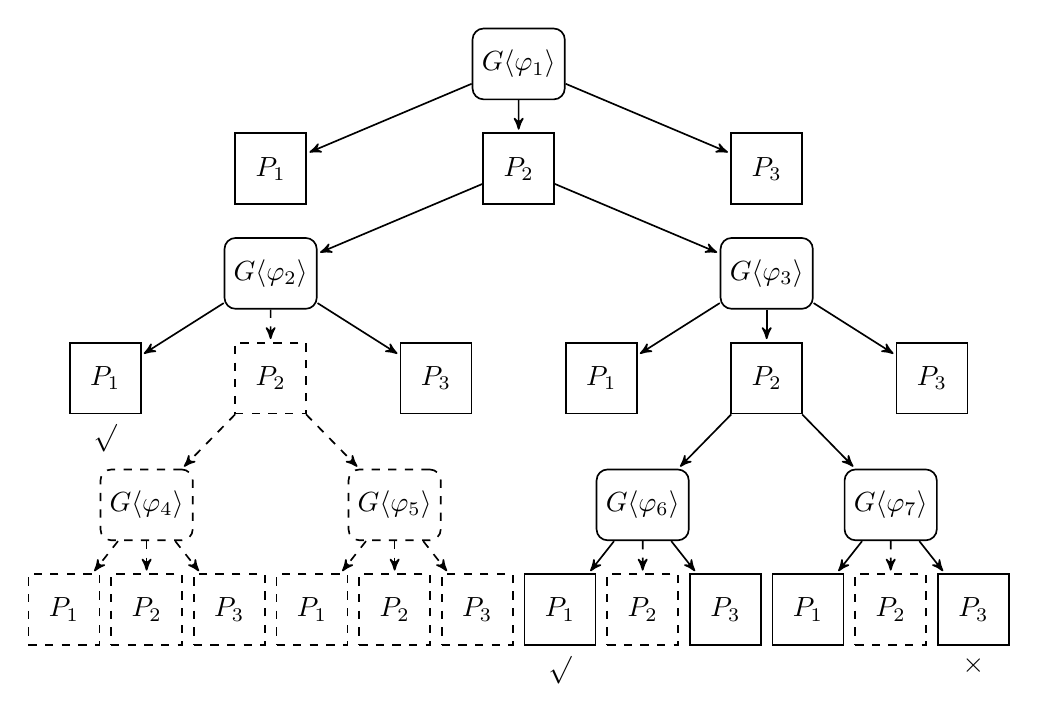
\begin{tikzpicture}[scale=0.7]
\tikzstyle{txt}=[scale=1.0]
\tikzstyle{succ}=[label=below:$\surd$]
\tikzstyle{fail}=[label=below:$\times$]
\tikzstyle{planbox}=[draw,minimum height=0.9cm,minimum width=0.9cm]
\tikzstyle{goalbox}=[draw,rounded corners,minimum height=0.9cm,minimum width=1.0cm]
\tikzstyle{level 1}=[sibling distance=4.5cm,level distance=1.9cm] 
\tikzstyle{level 2}=[sibling distance=9.0cm,level distance=1.9cm] 
\tikzstyle{level 3}=[sibling distance=3.0cm,level distance=1.9cm]
\tikzstyle{level 4}=[sibling distance=4.5cm,level distance=2.3cm]
\tikzstyle{level 5}=[sibling distance=1.5cm,level distance=1.9cm]
\tikzstyle{level 6}=[sibling distance=1.3cm,level distance=1.9cm]

\node[goalbox,yshift=1cm] {$G\langle\varphi_1\rangle$}
	child {node[planbox] {$P_1$}}
	child {node[planbox] {$P_2$}
		child {node[goalbox] {$G\langle\varphi_2\rangle$}
			child {node[planbox,succ] {$P_1$}}
			child[dashed] {node[planbox] {$P_2$}
				child {node[goalbox] {$G\langle\varphi_4\rangle$}
					child {node[planbox] {$P_1$}}
					child {node[planbox] {$P_2$}}
					child {node[planbox] {$P_3$}}
				}
				child {node[goalbox] {$G\langle\varphi_5\rangle$}
					child {node[planbox] {$P_1$}}
					child {node[planbox] {$P_2$}}
					child {node[planbox] {$P_3$}}
				}
			}
			child {node[planbox] {$P_3$}}
		}
		child {node[goalbox] {$G\langle\varphi_3\rangle$}
			child {node[planbox] {$P_1$}}
			child {node[planbox] {$P_2$}
				child {node[goalbox] {$G\langle\varphi_6\rangle$}
					child {node[planbox,succ] {$P_1$}}
					child[dashed] {node[planbox] {$P_2$}}
					child {node[planbox] {$P_3$}}
				}
				child {node[goalbox] {$G\langle\varphi_7\rangle$}
					child {node[planbox] {$P_1$}}
					child[dashed] {node[planbox] {$P_2$}}
					child {node[planbox,fail] {$P_3$}}
				}
			}
			child {node[planbox] {$P_3$}}
		}
	}
	child {node[planbox] {$P_3$}}
;

\end{tikzpicture}

}
\end{center}
\caption{Goal-plan hierarchy $\T_2$ containing a single goal type $G\langle\rangle$ handled by three plans $P_1$, $P_2$ and $P_3$. Here plan $P_2$ posts two instances of $G\langle\rangle$ resulting in recursion. Two levels of recursive unfolding are shown. Dashed $P_2$ nodes indicate roots of unexplored recursive sub-trees.}
\label{fig:unfolding}
\end{figure}

Consider the example BDI goal-plan hierarchy $\T_2$ of Figure \ref{fig:unfolding}. The structure has just a single event-goal type $G\langle\rangle$ and three options to handle it, one of which ($P_2$) in turn posts two instances of the same event-goal type $G\langle\rangle$. In this way, the only plans that take an action in the environment are $P_1$ and $P_3$. The figure highlights an execution trace as follows: \[
\lambda=G\langle\varphi_1\rangle[P_2:w_1] \cdot G\langle\varphi_2\rangle[P_1:w_1] \cdot G\langle\varphi_3\rangle[P_2:w_2] \cdot G\langle\varphi_6\rangle[P_1:w_2] \cdot G\langle\varphi_7\rangle[P_3:w_3].
\]

The first choice in the execution results in the selection of plan $P_2$ to handle event-goal instance $G\langle\varphi_1\rangle$ in a given world $w_1$. Plan $P_2$ in turn immediately posts the event-goal instance $G\langle\varphi_2\rangle$ that is successfully handled by the non-recursive node $P_1$. Plan $P_2$ then posts the second event-goal instance $G\langle\varphi_3\rangle$, which then is handled by itself in a recursive manner.  The outcome is that $\lambda$ traces a path that involves the successive execution of leaf plan $P_1$ for event-goal $G\langle\varphi_2\rangle$ followed by another execution of $P_1$ this time for event-goal $G\langle\varphi_6\rangle$, and finally terminates in the failure of leaf plan $P_3$ for event-goal $G\langle\varphi_7\rangle$. 

Note that if plan $P_2$ had instead been selected to handle $G\langle\varphi_7\rangle$ then a deeper recursive call would have ensued. Similarly if earlier in the execution trace plan $P_2$ was selected to handle event-goal $G\langle\varphi_2\rangle$ then a different recursive sub-tree (shown in Figure \ref{fig:unfolding} as dotted nodes under $G\langle\varphi_2\rangle$) would have unfolded.

The immediate implication of a recursive goal-plan structure is that the size of the hierarchy is no longer static but instead unfolds in a dynamic manner. The issue stems from the fact that the recursion is \textit{unbounded} because the context conditions that cause the recursion to terminate are initially unknown. So in order to know the context conditions we must recursively explore, but in doing so we risk an infinite recursive call because the context conditions that ought to guide the recursive exploration towards termination are unknown. This means that we may never find the ``bottom'' or leaf nodes. This has implications for any \textit{bottom-up} strategies. For instance, our conservative recording approach of \cite{Airiau:IJAT:09} and the coverage-based confidence measure of \cite{Singh:AAMAS10} both suffer from this problem. Interestingly, the simpler aggressive recording approach is not impacted by recursion as it does not consider the goal-plan structure . 

We will now focus on how the coverage-based confidence measure of \cite{Singh:AAMAS10} may be extended for use in recursive hierarchies.

\subsubsection{Calculating Coverage for Recursive Structures}

Since coverage is concerned with the number of paths {below} a plan in the goal-pplan hierarchy, then one way to interpret this for recursive structures is to treat all recursive goals simply as sub-trees in a static structure. Conceptually, this recursive unfolding of the structure is perfectly compatible with the coverage notion. 

Consider again the goal-plan structure $\T_2$ in Figure \ref{fig:unfolding} that shows the unfolding of the hierarchy for two levels of recursion. For the purpose of coverage calculations in this case, the three plans under each goal-event $G\langle\varphi_{4\ldots7}\rangle$ can be seen as having $[1,1,1]$ paths, plans under event-goals $G\langle\varphi_{2\ldots3}\rangle$ as having $[1,9,1]$ paths, and finally plans under $G\langle\varphi_1\rangle$ as having $[1,121,1]$ paths below.

The first difficulty with this reasoning, however, is that in fact the actual number of recursive unfoldings possible starting at $G\langle\varphi_1\rangle$ (or any other $G\langle\rangle$ for that matter) are \textit{infinite}. The only reason we are able to compute paths for structure $\T_2$ is because we have $bounded$ the recursion to a maximum of two levels.

It follows then that wherever a recursive structure applies and the coverage-based confidence measure is to be used, then a maximum recursion value must always be supplied. This may not be an unrealistic given that the domain expert will usually have some idea of how much recursion is sufficient, and as long as they provide a value that is sufficiently large for the domain then we have a valid case for computing coverage.

A second difficulty in this treatment of coverage is that the number of paths is exponential in the recursion number. For instance, in structure $\T_2$ in Figure \ref{fig:unfolding} the number of paths below $P_2$ for a progressively increasing recursion number is the series $[1, 9, 121, 15129, 228947161, \ldots]$. So within four levels of recursion, the number of paths below $P_2$ exceeds $228$ million.

Dhirendra says: Hmm.. one way to handle recursion would be to treat all recursive plans as \textit{leaf} nodes. This will enable coverage and stability to function in recursive domains ``as is''. Also all previous claims about coverage/stability will be preserved. Maybe this treatment of recursion makes more sense than bounded unfolding?!?

%Simplifications: Only single level goal recursion allowed ie G1->P1->G1 and not  G1->P1->G2->P2->G. Also no information of Gs in the system so only the parent goal recursion is tracked.

%\subsubsection{Discussion}
%Can we calculate $c_P(w,r)$ for any r if we have witnessed one r? 


%%%%%%%%%%%%%%%%%%%%%%%%%%%%%%%%%%%%%%%%%%%%%%%%%%%%
% \section{Two Approaches to Context Learning}\label{sec:context_learning}
\section{Context Learning: 2 Approaches}\label{sec:context_learning}
%%%%%%%%%%%%%%%%%%%%%%%%%%%%%%%%%%%%%%%%%%%%%%%%%%%%

\newcommand{\success}{\mbox{\emph{succ}}}
\newcommand{\failure}{\mbox{\emph{fail}}}

With the classical BDI programming framework extended with decision trees and a
probabilistic plan selection scheme, we are now ready to develop mechanisms for
learning context decision trees
%and hopefully improving over time the selection
%of plans based on experience.
based on online experiences, in order to improve plan selection over time.
% %
To that end, in this section, we explore two approaches for learning the context
condition of plans.



Recall that our objective is to learn which plans are best for achieving
a particular goal event in the various world states that may ensue. Given that,
in this work, we have no measure of cost for plans,\footnote{This could also be a
useful addition, but is not part of standard BDI programming languages.} a good
plan for a given world state is simply one which (usually) succeeds in such
state. In order to learn the context decision tree for a plan, the agent keeps
track of previous experiences she has had when running the plan in question. More
precisely, if a plan $P$ is tried in world state $w$ with certain outcome $o \in
\{\success,\failure\}$, the agent may record the tuple $\tuple{w,o}$ as part of
the training set for plan $P$.
% %
Interestingly, while it is always meaningful to record successful executions,
some failures may not be worth recording. Based on this observation, we shall
develop and compare two different algorithms that differ on how past experiences
are taken into account by the agent. Before then, though, let us explain better
this issue by means of an example.
 

\begin{figure}[t]
\begin{center}
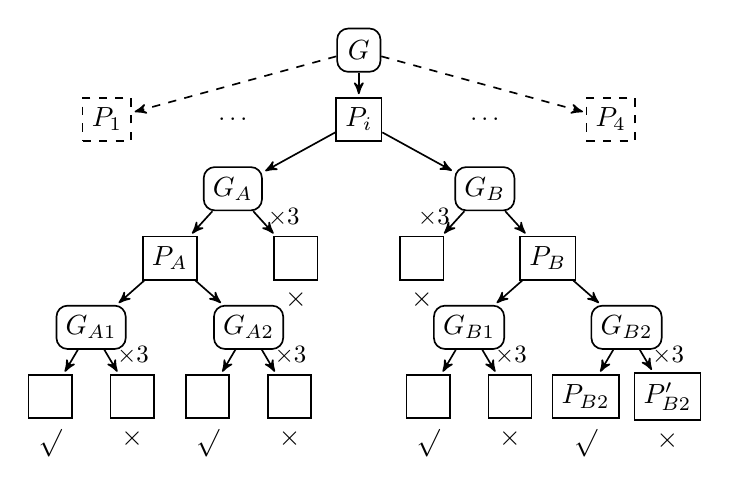
\begin{tikzpicture}[scale=0.8,level distance=1.1cm]
\tikzstyle{txt}=[scale=.9]
\tikzstyle{succ}=[label=below:$\surd$]
\tikzstyle{fail}=[label=below:$\times$]

\tikzstyle{planbox}=[draw,minimum height=0.55cm,minimum width=0.55cm]
\tikzstyle{goalbox}=[draw,rounded corners,minimum height=0.55cm,minimum width=0.55cm]

	
\tikzstyle{level 1}=[sibling distance=4.0cm] 
\tikzstyle{level 2}=[sibling distance=4cm] 
\tikzstyle{level 3}=[sibling distance=2cm]
\tikzstyle{level 4}=[sibling distance=2.5cm]
\tikzstyle{level 5}=[sibling distance=1.3cm]

\node[goalbox,yshift=1cm,solid] (T) {$G$}
	child[dashed] {node[planbox] (P1) {$P_1$}}
	child[solid] {node[planbox] (Pi) {$P_i$}
		child {node[goalbox] {$G_A$}
			child {node[planbox] {$P_{A}$}
				child {node[goalbox] {$G_{A1}$}
					child {node[planbox,succ] {$\phantom{P}$}}
					child {node[planbox,fail] {$\phantom{P}$} 
					edge from parent node[txt,right,near start] {$\times 3$}
					}
				}
				child {node[goalbox] {$G_{A2}$}
					child {node[planbox,succ] {$\phantom{P}$}}
					child {node[planbox,fail] {$\phantom{P}$} 
						edge from parent node[txt,right,near start] {$\times 3$}
					}
				}
			}
			child {node[planbox,fail] {$\phantom{P}$} 
				edge from parent node[txt,right,near start] {$\times 3$}
			}
		}
		child {node[goalbox] {$G_{B}$}
			child {node[planbox,fail] {$\phantom{P}$}
				edge from parent node[txt,left,near start] {$\times 3$}
			}
			child {node[planbox] {$P_B$}
				child {node[goalbox] {$G_{B1}$}
					child {node[planbox,succ] {$\phantom{P}$}}
					child {node[planbox,fail] {$\phantom{P}$}
						edge from parent node[txt,right,near start] {$\times 3$}
					}
				}
				child {node[goalbox] {$G_{B2}$}
					child {node[planbox,succ] {$P_{B2}$}}
					child {node[planbox,fail] {$P_{B2}'$}
						edge from parent node[txt,right,near start] {$\times 3$}
					}
				}
			}
		}
	}
	child[dashed] {node[planbox] (P4) {$P_4$}}
;
\node[txt] at ($ (P1)!.5!(Pi) $) {$\ldots$};
\node[txt] at ($ (Pi)!.5!(P4) $) {$\ldots$};

\end{tikzpicture}

\end{center}
\caption{Goal-Plan hierarchy $\T_3$. There are $2^4$ worlds whose solutions are
distributed evenly in each of the $4$ top level plans. Successful execution trace
is of length $4$. Within each sub-tree $P_i$ \BUL\ is expected to perform better
for a given world, but it suffers in the number of worlds. Overall, \CL\ and \BUL\
perform equally well in this structure.}
\label{fig:T3}
\end{figure}



Consider the example in Figure \ref{fig:T3}.
% %
Suppose that in some execution, plan $P_i$, for some $i \in \{1,\ldots,4\}$, is
selected in order to resolve top-goal $G$ in some world state $w_1$. The plan
involves, in turn, the successful resolution of sequential goals $G_A$ and $G_B$.
Suppose further that subgoal $G_A$ has been resolved successfully, yielding new
state $w_2$, and that plan $P_B$ has been chosen next to try and achieve the
second subgoal $G_B$.
% %
Suppose next that the first subgoal of plan $P_B$, namely $G_{B1}$ has been
successfully resolved, yielding new state $w_3$, but that the non-working plan
$P_{B2}'$ for subgoal $G_{B2}$ is selected in $w_3$ and execution thus
\emph{fails}.
% %
As there is no failure recovery, this failure will be propagated upwards in the
hierarchy, causing goals $G_{B2}$ as well as $G_B$ and top-level goal $G$ itself
to fail.
% %
First of all, the failure (in world state $w_3$) must be recorded in the decision
tree of the plan where the failure originated, namely, plan $P_{B2}'$. 
%Such plan is in fact ``low-level,'' in that it has no subgoals and thus interacts with the
%external world directly. Hence, all we can expect is to learn such interaction
%over time.
Such bottom-level plans have no subgoals, so they interact with the
external world directly, and over time we can expect to learn such interactions.
% %
On the other hand, as we will show below, it is not so clear  whether the failure should also be
recorded in the decision trees for plans higher up in the hierarchy (e.g., plans
$P_B$ and $P_i$).






In order to discuss further \emph{which} data should be recorded \emph{where}, we
define the notion of an \textit{active execution trace}, as a sequence of the
form $G_0[P_0:w_0] \cdot G_1[P_1:w_1] \cdot \ldots \cdot G_n[P_n:w_n]$, which
represents the sequence of currently active goals, along with the plans which
have been selected to achieve each of them, and the world state in which the
selection was made---plan $P_i$ has been selected in world state $w_i$ in order
to achieve the $i$-th active subgoal $G_i$.
% %
In our example, the trace at the moment of failure is as follows: \[
\lambda=G[P_i:w_1] \cdot G_B[P_B:w_2] \cdot G_{B2}[P_{B2}':w_3]. \]


So, when the final goal of $\lambda$ fails, namely $G_{B2}$, it is clear that the
decision tree of the plan being used to achieve such goal ought to be updated,
and a failure should be recorded for the world state $w_3$ against 
the decision tree attached to plan $P_{B2}'$.  
%%
By recording every outcome for the lowest plans, i.e., plans with no subgoals,
the system eventually learns how such plans perform in the environment.
%%
% Although it may be the case
% that the plan usually succeeds in the situation in which it was chosen, and failure is
% simply due to some non-determinism (or in the general case, actions of other
% agents, interactions, etc.), there is no way to determine this and the learning
% process will eventually recognise such cases as ``noise.''
% %

What is more difficult to determine is whether the decision trees of plans
associated with \emph{earlier goals} in $\lambda$ should also be updated.
% %
More concretely, should failure cases in world states $w_2$ and $w_1$ be recorded
against plans $P_B$ and $P_i$, respectively?
% %
The point is that it is conceivable that the failure of subgoal $G_{B2}$ in plan
$P_B$, for instance, could indeed have been avoided, had the alternative plan
$P_{B2}$, been chosen instead. Therefore, recording a failure against plan $P_B$
would not be justified---it is not true that plan $P_{B}$ is a ``bad'' one
in world state $w_2$.
% %
Informally, one could argue that it is more appropiate to \emph{wait} before
recording failures against a plan until one is reasonably confident that
subsequent choices down the goal-plan tree hierarchy were ``well informed.'' In
our case, if the agent knows that the plan selection for goal $G_{B2}$ was as
good and informed as possible, then recording the failure for world $w_2$ in plan
$P_B$ would also be justified. Similarly, if the agent considers that the plan
selection for subgoal $G_B$ was an informed choice, then recording the failure
for world $w_1$ against $P_i$'s decision tree would be justified too.


\newcommand{\procedurefont}[1]{\mathsf{#1}}
\newcommand{\StableGoal}{\procedurefont{StableGoal}}
\newcommand{\RecordTrace}{\procedurefont{RecordFailedTrace}}
\newcommand{\RecordWorldDT}{\procedurefont{RecordWorldDT}}




The judgment as to whether plan choices were sufficiently ``well informed,'' is
however not a trivial one.  A plan $P$ is considered to be \emph{stable} for a
particular world state $w$ if the rate of success of $P$ in $w$ is changing below
a certain threshold $\epsilon$. In such a case, the agent can start to build
confidence about the applicability level of $P$. The stability notion extends to
goals as follows: a goal is considered \emph{stable} for world state $w$ if all
its relevant plans are stable for $w$.
% %
When a goal is stable, we regard the plan selection for such goal as a ``well
informed'' one. Thus, a failure is recorded in the plan for a given world if the subgoal that failed is stable for the respective world in which it was resolved. In our example, we
record the failure in plan $P_B$ ($P_i$) if goal $G_{B2}$ ($G_B$) is deemed stable
in world state $w_3$ ($w_2$), that is, if the selection of option $P_{B2}'$
($P_B$) was an informed one.



The $\RecordTrace$ algorithm below shows how a failed execution run $\lambda$ is
recorded. Function
$\StableGoal(G,w,k,\epsilon)$ returns true iff goal $G$ is considered \textit{stable} for world state $w$, for success rate change 
threshold $0 < \epsilon \leq 1$ and minimal number of executions $k
\geq 0$.
%
The algorithm starts by recording the failure against the last plan $P_n$ in the
trace.
% %
Next, if the choice of executing plan $P_n$ to achieve goal $G_n$ was deemed an
informed one (that is, goal $G_n$ was stable for $w_n$), then the procedure
should be repeated for the previous goal-plan nodes, if any.
% %
If, on the other hand, the last goal $G_n$ in the trace is not considered stable
enough, the procedure terminates and no more failure data is assimilated.
% %
Observe that, in order to update the decision tree of a certain plan that was
chosen along the execution, it has to be the case that the (failed) decisions
taken during execution must have all been informed ones.
 
 \renewcommand{\algorithmiccomment}[1]{\hfill \texttt{\small // #1}}
 \newcommand{\assign}{\mbox{:=\ }}
 \begin{algorithm}[h]
	\caption{$\RecordTrace(\lambda,k,\epsilon)$}\label{algo:record_failed_exec}
	\label{alg:NDS}
  \begin{algorithmic}[1]
    \REQUIRE $\lambda=G_0[P_0:w_0] \cdot \ldots \cdot G_n[P_n:w_n]$; $k\geq0$;
    $\epsilon > 0$ \ENSURE Propagates DT updates for plans

	\STATE $\RecordWorldDT(P_n,w_n,\failure)$

    \IF{$\StableGoal(G_n,w_n,k,\epsilon) \land |\lambda|>1$}
    	 \STATE $\lambda' \assign G_0[P_0:w_0] \cdot \ldots \cdot
    				G_{n-1}[P_{n-1}:w_{n-1}]$
    	\STATE $\RecordTrace(\lambda',k,\epsilon)$ \COMMENT{recursive call}
    \ENDIF
  \end{algorithmic}
\end{algorithm}

 



So, in the remainder of the paper, we shall consider two learning approaches
compatible with the framework developed in the previous section. The first, which
we call \emph{aggressive concurrent learning} (\CL), corresponds to the more
traditional approach where all data is always assimilated by the learner, that
is, we take $\epsilon = 1$ and $k = 0$. In other words, every plan and every goal
is always considered stable and, as a result, a failure in a plan is always
recorded. The assumption is that misleading information, as discussed above, will
eventually disappear as noise.
% %
The second one, which we refer to as \emph{bottom-up learning} (\BUL), is more
cautious and records a failure execution experience when the success rate has stabilised i.e. is not changing by more than $\epsilon$.
In our work, we have taken
$\epsilon = 0.3$ and $k = 3$, that is, the context condition of a plan is
considered stable (for a world state) if at least $3$ past execution experiences
have been recorded 
%and the rate of success has lately been changing less than $0.3$.
and the change in the rate of success over the last two experiences is less than $0.3$.
% %
Note that the lower $\epsilon$ is and the higher $k$ is, the more conservative
the agent is in considering its decisions ``well informed.''

In the following section, we shall explore these two approaches against
different programs with different structures.






%%%%%%%%%%%%%%%%%%%%%%%%%%%%%%%%%%%%%%%%%%%%%%%%%%%%
\section{Experimental Results}\label{sec:experiments}
%%%%%%%%%%%%%%%%%%%%%%%%%%%%%%%%%%%%%%%%%%%%%%%%%%%%

In order to explore the difference between \BUL\ and \CL, we set up testbed
programs composed of several goals and plans combined in a hierarchical manner
and yielding goal-plan tree structures of different shapes.\footnote{We have
implemented the learning agent system in the \JACK\ BDI platform
\cite{Busetta99jack}. The fact that \JACK\ is a Java-based system and
provides powerful meta-level reasoning capabilities, allows us to integrate \weka\ and
probabilistic plan-selection mechanisms with not much effort. Nonetheless, all
the results are independent on this and any other BDI agent system could
have been used.}
% %
In particular, we crafted goal-plan tree structures representing different
cases of BDI programs with one main top-level goal, i.e., the event to
be resolved. In addition, for each structure there is always a way of addressing the main goal, i.e. there is at
least one successful execution of the top-level event provided the right plan
choices are made. Observe that such successful (plan) choices are different
for different world states.
% , as know-how information is generally predicated on the situation it is
% applied in. %
When it comes to describing the possible (observable) world states, we have used
a set of logical (binary) propositions, representing the so-called fluents or
features of the environment that are observable to the agent (e.g., fluent
proposition $\mathit{DoorLocked}$ states whether the door is believed open or
not).
% %
Finally, we assume the agent is acting in a non-deterministic environment in
which actions that are expected to succeed may still fail with some
probability. In our experiments we assign a $0.1$ probability of
unaccounted failure to all actions.\footnote{See Discussion section on how our
results generalize to a framework with world state built from non-binary fluents
and with more complex accounts for stochastic actions.}
% %




The experiments consisted in posting the top-level goal repetitively under random
world states, running the corresponding  BDI learning agent, and finally
recording whether the execution terminated successfully or not.
% %
%We calculated the average rate of success of the goal every some fixed
%number of iterations (in our case $20$), and investigated how such rate evolved
%as the agent refined the context condition of plans.
We calculate the average rate of success of the goal by first averaging the
results at each time step over $5$ runs of the same experiment, and then
smoothing using a moving average of the previous 100 time steps to get the trends
reported in the figures.
% %%
We ran the tests with both a \BUL-based agent and a \CL-based agent, ensuring the
same sampling of random world states for each.

\begin{figure}[t]
\begin{center}
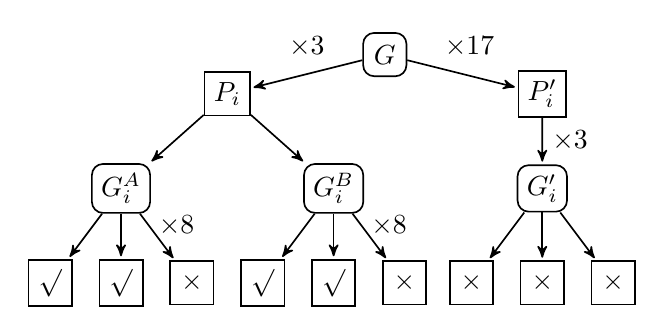
\begin{tikzpicture}[level distance=1.2cm]

\tikzstyle{planbox}=[draw,minimum height=0.55cm,minimum width=0.55cm]
\tikzstyle{goalbox}=[draw,rounded corners,minimum height=0.55cm,minimum width=0.55cm]

\tikzstyle{level 1}=[sibling distance=4cm,level distance=0.5cm] 
\tikzstyle{level 2}=[sibling distance=2.7cm,level distance=1.2cm]
\tikzstyle{level 3}=[sibling distance=.9cm]
\tikzstyle{level 4}=[sibling distance=1cm]

\node[goalbox] (T) {$G$}
   child[solid] {node[planbox] (1) {$P_i$}
      	child {node[goalbox] (11) {$G_i^A$}
			child {node[planbox] {$\surd$}
			}
			child {node[planbox] {$\surd$}
			}
			child {node[planbox] {$\times$}
				edge from parent node[right,near start] {$\times 8$}
			}
	  	}
      	child {node[goalbox] (11) {$G_i^B$}
			child {node[planbox] {$\surd$}
			}
			child {node[planbox] {$\surd$}
			}
			child {node[planbox] {$\times$}
				edge from parent node[right,near start] {$\times 8$}
			}
	  	}
	edge from parent node[above left, near start] {$\times 3$}
   }
   child[solid] {node[planbox] (2) {$P_i'$}
      child {node[goalbox] (22) {$G_i'$} 
	child {node[planbox] {$\times$}}
	child {node[planbox] {$\times$}}
	child {node[planbox] {$\times$}}
	edge from parent node[right] {$\times 3$}
	}
   edge from parent node[above right,near start] {$\times 17$}};

% \draw (T) -- (1) node (aux1) [coordinate,midway]{};
% \draw (T) -- (2) node (aux2) [coordinate,midway]{};
% \draw (aux1) .. controls +(0.3,-0.3) and +(-0.3,-0.3).. (aux2)
% 			node[midway,above] {OR};

% \draw (1) -- (11) node (aux21) [coordinate,midway]{};
% \draw (1) -- (12) node (aux23) [coordinate,midway]{};
% \draw (aux21) .. controls +(0.25,-0.25) and +(-0.25,-0.25).. (aux23)
% 			node[midway,above] {AND};

% \node[below left of=T,text width=2cm,xshift=-3cm] (label)
% 		{$P_i$: plan \\ $G_i$: goals \\ $SG_i$: sub-goals};
\end{tikzpicture}

\end{center}
\caption{Goal-plan tree structure $\T_1$. To succeed, an agent needs 
to make three correct choices, including selecting  $P_i$ at the
top-level. The solutions to $2^3$ worlds are distributed evenly in the $3$ plans 
$P_i$. \CL\ outperforms \BUL\ in this structure.}
\label{fig:T1}
\end{figure}


From our set of experiments, we have selected three hierarchical structures that
best illustrate the results that we have obtained, namely:
% %
\begin{description}
\item[(Tree $\T_1$; Figure~\ref{fig:T1})] For each world state, the
goal has a few plans that can succeed (plans $P_i$), but many other options of comparable
complexity that are bound to fail (plans $P_i'$).\footnote{Here, plan
complexity refers to the size of the fully expanded plan, as represented
by the number of levels of abstraction and the numbers of goals at each level.
The key factor is the number of abstraction levels---abstract plans are not in
themselves complex.}
%%
Under this type of structure, an \CL-based agent will generally perform better 
than an agent using the learning \BUL\ approach.

\item[(Tree $\T_2$; Figure~\ref{fig:T2})] For each world state, the goal has
one plan that can succeed (plan $P$), and a few others that would fail.
However, the plan containing the solution is of substantially
higher-complexity.
%%
In this structure, a \BUL-based agent will outperform an \CL-based one.
% A structure in which \BUL\ is
% expected to have important advantages over \CL, since the latter may wrongly consider a
% top-level plan as a failing plan whereas there is a solution encoded
% under it. 

\item[(Tree $\T_3$; Figure~\ref{fig:T3})] This tree represents a ``balanced''
structure that ends up providing different advantages for both \BUL\ and \CL\ in
different parts of the tree.
\end{description}


% In summary, we found that whereas the agent performance under the \BUL\ and \CL\
% approaches is comparable on the first and third cases, the \BUL\ scheme provides
% substantial benefits in the second case. What is more important, if we consider
% agents that may choose not to consider a plan at all when its chances of success
% are believed very low, then the \CL\ approach collapses completely whereas the
% \BUL\ is robust enough to maintain performance.

% For lack of space, we shall only give the form of tree $\T_1$ and informally
% explain the characteristics of the other two.

Let us next discuss each of the plan-goal structures and how the performance of
\BUL-based and \CL-based agents compare.


Under a structure like $\T_1$, the agent basically has several options of
comparable complexity to resolve the top-level goal $G$ in a certain
world state. In $\T_1$ there are $20$ options.
However, most such options ($17$ in our example, plans $P_i'$)
inevitably lead to failure.  
% %
The benefit of using the \CL\ approach comes from the fact that the agent will
decrease the probability of selecting each of those $17$ failing plans as soon as
they fail for the first time. In contrast, \BUL\ requires multiple failed
experiences of each of those ``bad'' top-level options before decreasing their
probability of selection because each subgoal of each plan $P_i'$ must
be stable before that $P_i'$ is updated. 
%---to update the decision tree of each plan $P_i'$, \BUL\
%requires each of the three subgoals of that plan to be ``stable.''
% %%
The \CL\ agent did indeed perform better in our experiments, in that it
achieved better success rate earlier as shown in Figure~\ref{fig:T1_result}.
% %
% The \CL\ approach reaches $50\%$ success after $600$ iterations,
% whereas it takes more than double that for \BUL.
%%
Observe that, eventually, both approaches will yield optimal
performance.\footnote{Optimal performance in this case amounts to a success rate
of $81\%$, as the environment fails with probability $.1$ for every (working) action and each
successful execution involves the performance of two actions (leaf plans consist
of single actions).}


\begin{figure}[t]
\begin{center}
%!TEX root = ../dsingh-aamas10.tex
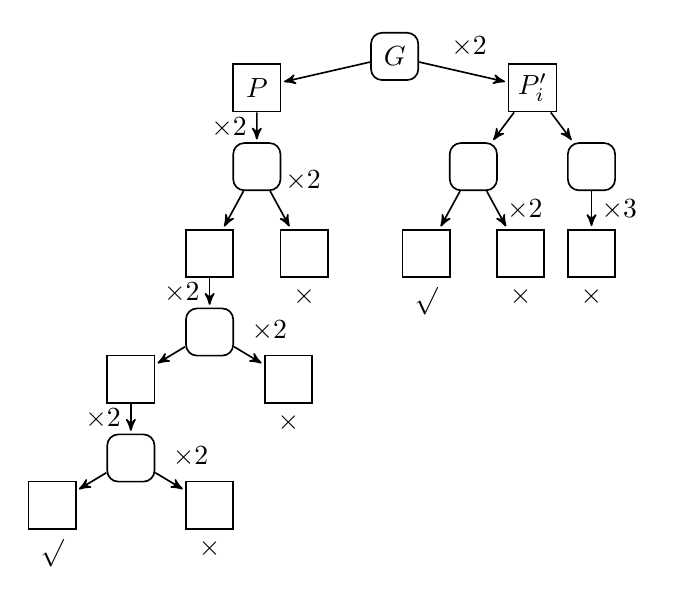
\begin{tikzpicture}[level distance=1.2cm]
\tikzstyle{txt}=[scale=.9]

\tikzstyle{succ}=[label=below:$\surd$]
\tikzstyle{fail}=[label=below:$\times$]


\tikzstyle{planbox}=[draw,minimum height=0.6cm,minimum width=0.6cm]
\tikzstyle{goalbox}=[draw,rounded corners,minimum height=0.6cm,minimum width=0.6cm]

\tikzstyle{level 1}=[sibling distance=3.5cm,level distance=0.4cm] 
\tikzstyle{level 2}=[sibling distance=1.5cm,level distance=1.0cm]
\tikzstyle{level 3}=[sibling distance=1.2cm,level distance=1.1cm]
\tikzstyle{level 4}=[sibling distance=1.2cm,level distance=1.0cm]
\tikzstyle{level 5}=[sibling distance=2.0cm,level distance=0.6cm]
\tikzstyle{level 6}=[sibling distance=1.2cm,level distance=1.0cm]
\tikzstyle{level 7}=[sibling distance=2.0cm,level distance=0.6cm]
\tikzstyle{level 8}=[sibling distance=1.2cm,level distance=1.0cm]

\node[goalbox] (T) {$G$}
   child[solid] {node[planbox] (1) {$P$}
      child {node[goalbox] (11) {\phantom{$G$}}
		child {node[planbox] {\phantom{$P$}}
			child {node[goalbox] {\phantom{$G$}}
				child {node[planbox] {\phantom{$P$}}
					child {node[goalbox] {\phantom{$G$}}
						child {node[planbox,succ] {\phantom{$P$}}}
						child {node[planbox,fail] {\phantom{$P$}}
							edge from parent node[above right,near start] {$\times 2$}
						}
						edge from parent node[left] {$\times 2$}
					}
				}
				child {node[planbox,fail] {$\phantom{P}$}
					edge from parent node[above right,near start] {$\times 2$}
				}
		               edge from parent node[left] {$\times 2$}
			}
		}
		child {node[planbox,fail] {\phantom{$P$}}
			edge from parent node[above right,near start] {$\times 2$}
		}
               edge from parent node[left] {$\times 2$}
	}
   }
   child[solid] {node[planbox] (2) {$P_i'$}
      	child {node[goalbox] (11) {\phantom{$G$}}
			child {node[planbox,succ] {$\phantom{P}$}}
			child {node[planbox,fail] {$\phantom{P}$} 
		               edge from parent node[right] {$\times 2$}
			}
	}
      	child {node[goalbox] {\phantom{$G$}}
			child {node[planbox,fail] {$\phantom{P}$} 
		               edge from parent node[right] {$\times 3$}
			}
	}
	edge from parent node[above right, near start] {$\times 2$}
};
\end{tikzpicture}



\end{center}
\caption{Goal-plan tree hierarchical structure $\T_2$. Successful execution requires numerous correct choices including $8$ correct action nodes. The solutions to $2^3$ worlds are in the plan labelled $P$. \BUL\ outperforms \CL\ in this structure.}
\label{fig:T2}
\end{figure}


\begin{figure*}[t]
\begin{center}
\subfigure[Structure $\T_1$]{\label{fig:T1_result}
%!TEX root = ../dsingh-aamas10-poster.tex
\begin{tikzpicture}[x= 0.008cm,y=9cm]
	\definecolor{darkblue}{rgb}{0.1,0.1,0.5}
	\definecolor{darkred}{rgb}{0.8,0.0,0.1}
    % Draw the axes and grid lines
    \draw[-] (0,0) -- (0,1) -- (2000,1) -- (2000,0) -- cycle; 
    \draw[-,thin, dotted, ystep=0.2, xstep=2000] (0,0) grid (2000,1);
    \foreach \x in {500, 1000, 1500}  \draw [-,xshift=0](\x,4pt) -- (\x,-1pt);
    \foreach \y in {0.0,0.2,0.4,0.6,0.8,1.0}  \draw [-,yshift=0](4pt,\y) -- (-1pt,\y);
    \foreach \x/\xtext in {500/500, 1000/1000, 1500/1500} \node at (\x,0) [below] {\xtext};
    \foreach \y/\ytext in {0.0,0.2,0.4,0.6,0.8,1.0}  \node at (0,\y) [left] {\ytext};
    \node at (0,1.15) {Success};
    \node at (1650,0.1) {Iterations};
    \draw[-,darkred] plot[mark=x,mark size=10,mark options={color=darkred}] 
			file {figs/data/test01v3gm.CP.tikzdata};
    \draw[-,darkblue] plot[mark=o,mark size=6,mark options={color=darkblue}] 
			file {figs/data/test01v3gm.SP.tikzdata};
    % Also draw the expected convergence: 0.9^4 actions=0.6561
    \draw[dashed,-,yshift=0](0,0.81) -- (2000,0.81);
	\node at (2300,0.5) {$\mathcal{T}1$};
\end{tikzpicture}

}
\qquad
\subfigure[Structure $\T_2$]{\label{fig:T2_result}
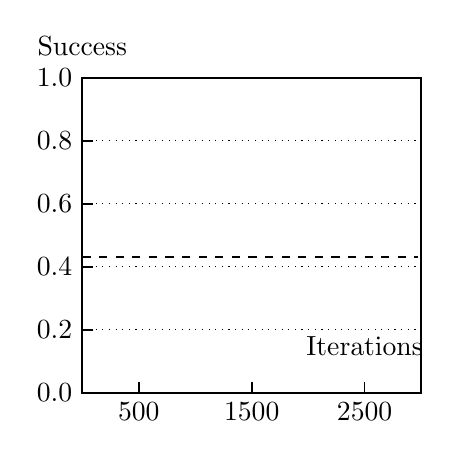
\begin{tikzpicture}[x=0.00143cm,y=4cm]
    % Draw the axes and grid lines
    \draw[-] (0,0) -- (0,1) -- (3000,1) -- (3000,0) -- cycle; 
    \draw[-,thin, dotted, ystep=0.2, xstep=3000] (0,0) grid (3000,1);
    \foreach \x in {500, 1500, 2500}  \draw [-,xshift=0](\x,4pt) -- (\x,-1pt);
    \foreach \y in {0.0,0.2,0.4,0.6,0.8,1.0}  \draw [-,yshift=0](4pt,\y) -- (-1pt,\y);
    \foreach \x/\xtext in {500/500, 1500/1500, 2500/2500} \node at (\x,0) [below] {$\xtext$};
    \foreach \y/\ytext in {0.0,0.2,0.4,0.6,0.8,1.0}  \node at (0,\y) [left] {$\ytext$};
    \node at (0,1.1) {Success};
    \node at (2500,0.15) {Iterations};
    \draw[-] plot[mark=triangle,gray,mark size=3,mark options={color=gray}] 
			file {data/test05v3gm.CP.tikzdata};
    \draw[-] plot[mark=o,gray,mark size=2,mark options={color=gray}] 
			file {data/test05v3gm.SP.tikzdata};
    % Also draw the expected convergence: 0.9^8 actions=0.43046
    \draw[dashed,-,yshift=0](0,0.43046) -- (3000,0.43046);

\end{tikzpicture}

}
\qquad
\subfigure[Structure $\T_3$]{\label{fig:T3_result}
%!TEX root = ../dsingh-aamas10-poster.tex
\begin{tikzpicture}[x=0.0032cm,y=9cm]
    % Draw the axes and grid lines
    \draw[-] (0,0) -- (0,1) -- (5000,1) -- (5000,0) -- cycle; 
    \draw[-,thin, dotted, ystep=0.2, xstep=5000] (0,0) grid (5000,1);
    \foreach \x in {1000, 2500, 4000}  \draw [-,xshift=0](\x,4pt) -- (\x,-1pt);
    \foreach \y in {0.0,0.2,0.4,0.6,0.8,1.0}  \draw [-,yshift=0](4pt,\y) -- (-1pt,\y);
    \foreach \x/\xtext in {1000/1000, 2500/2500, 4000/4000} \node at (\x,0) [below] {\xtext};
    \foreach \y/\ytext in {0.0,0.2,0.4,0.6,0.8,1.0}  \node at (0,\y) [left] {\ytext};
    \node at (0,1.15) {Success};
    \node at (4150,0.1) {Iterations};
    \draw[-,red] plot[mark=x,mark size=10,mark options={color=red}] 
			file {figs/data/testImpactvars2.CP.tikzdata};
    \draw[-,blue] plot[mark=o,mark size=6,mark options={color=blue}] 
			file {figs/data/testImpactvars2.SP.tikzdata};
    % Also draw the expected convergence: 0.9^4 actions=0.6561
    \draw[dashed,-,yshift=0](0,0.6561) -- (5000,0.6561);
	\node at (5700,0.5) {$\mathcal{T}3$};

\end{tikzpicture}

}
\caption{Agent performance under \BUL\ (circles) and \CL\ (crosses) schemes.
Each point represents results from $5$ experiment runs using an averaging window
of $100$ samples. The dashed line represents optimal performance (Note that
outcomes are always $0$ or $1$ so more than expected consecutive successes may
seems like ``above'' optimal performance when averaged).}
\end{center}
\end{figure*}


Let us now analyse the goal-plan tree $\T_2$ shown in Figure~\ref{fig:T2}.
% %
Under such a structure, all successful executions are encoded in a complex plan,
in our case plan $P$. Other options that the agent may have (e.g., plans $P_i'$)
are of less complexity, but do not lead to solutions for resolving the
goal.\footnote{This is an extreme case for illustrative purposes. Of course the
simpler plans $P_i'$ would, in a real program, lead to a solution in some world
states or it would not make sense to include them. The same effect would however
arise if most world states had solutions only in a complex plan branch.}
% %
Because the plan containing the solution, namely $P$, is fairly complex, there
are many ways the agent may fail when exploring the decomposition of $P$. The
agent needs to make several correct choices to obtain a successful execution.
% %
Although we expected \BUL\ to yield better agent performance than \CL, the
difference was enormous in our experiments. Figure~\ref{fig:T2_result} shows that
while the \BUL\ approach achieves optimal performance, which amounts to slightly
over $40\%$ rate of success, in slightly more than $500$ iterations, the \CL\
scheme, requires more than $3000$ execution experiences. The reason is clear:
since there are more chances to fail plan $P$ initially, \CL\ marks this plan as
``bad,'' compared with the non-working plans $P_i'$. On the other hand, \BUL\
would not jump to the conclusion that $P$ is a ``bad'' plan even when failing it,
since it is aware that decisions made below $P$ were not sufficiently informed.
Consequently, plan $P$ will continue to be explored with \emph{equal} likelihood
to plans $P_i'$.
% %
This structure shows exactly the problem discussed in the previous section,
namely, the drawbacks of assuming that a plan is a bad option just because it
happened to fail, without consideration of the confidence in the choices made
below it.


Finally, consider the hierarchical structure $\T_3$ depicted in Figure
\ref{fig:T3}.
% %
In this case, the top-level goal $G$ has four relevant plans, which are all
``complex,'' that is, they all have several levels and multiple goals and plans.
However, given a world state, only one particular path in this hierarchy will
lead to a successful execution (of course, for different states, different
top-level plans may apply). Among other things, this means that at the top-level
the agent needs to select the right plan given the current world state. All 
other plans are bound to eventually fail.
% %
We argue that this is a common feature found in many BDI agent applications, in
that even though the agent has been programmed with several strategies for
resolving a goal, each one is crafted to cover uniquely a particular subset of
states. In other words, these are systems with low \emph{know-how} overlap.
% %
With respect to the two learning approaches we are considering, structure $\T_3$
provides advantages for both of them, in different parts of the tree. The \CL\
scheme is expected to learn faster the inadequacy of the non-working top-level
programs, whereas the \BUL\ would better explore, and find a solution, within the
working top-level plan. This balance is evident in Figure~\ref{fig:T3_result} 
where both approaches show comparable performance.




\subsection{Plan Applicability and Optimality}

So far, we have assumed that the agent considers all relevant plans
for a goal as also \emph{applicable}, even though some may have a very
low chance of success.
% %
This implies that, in contrast with standard BDI systems, our extended
learning BDI framework will \emph{always} select a plan among the relevant
options.
% %
Because executing a plan is often not cost-free in real systems, it is likely
that an adequate plan selection mechanism would in fact \emph{not} execute plans
with too low a probability of success. This, in turn, implies that the system
may, at some point, decide to fail a goal without even trying it, if it
considers that the high likelihood of failure does not justify the
cost of attempting any of the relevant plans.
%cost of failing at that point is preferable to expected
%benefits of executing some available plan.
%%
This is exactly what standard BDI systems do. When no applicable plan
is found for a certain event goal, that event goal is failed right away.


To understand the impact of applicability in our BDI learning framework, we
modified the probabilistic plan selection so that the agent does \emph{not} consider
plans whose chances of success are deemed below a threshold; in our case we set
this threshold to $0.2$.
% %
For simplicity, we  removed the non-determinism in the model of the
environment: actions either fail or succeed in each world state.

%The difference between \CL-based and \BUL-based agents performance when run with
%an applicability threshold could be striking
% %
Using the structure $\T_3$ we found that whereas the \BUL\ scheme maintains its
performance (and in fact may slightly improve due to truly failing leaf plans
being ruled out earlier), the \CL\ approach may not able to learn at all and
could end up eventually failing the top-level goal \emph{always}. This is
reported in Figure~\ref{fig:performance-applicability} (dotted lines).

The explanation for this undesirable behavior under \CL\ is as follows.
% %
Initially, the agent tries all top-level plans for the top-level goal, including
the ones containing potential successful executions. Because of their complexity,
the chance of finding a successful execution immediately is very low, and most
executions fail initially. With each failure, \CL\ decreases the feasibility of
all plans tried, including the top-level one.  After several failures, all plans
for the top-level goal eventually go below the applicability threshold of the
system (including the ``good'' plans). When that happens, the system has no more
applicable plans for the goal and will therefore fail it always.
% %
This behavior does not arise in the original system, because even if all plans
perform very poorly, the agent would always pick one anyway, the successful path
would be eventually be found, and the context decision trees of the plans
associated with such a path would then start ``recovering.''


The reason \BUL\ exhibits more robust behaviour here is that false negative
executions (i.e., failing executions of plans that do encode successful
runs) will \emph{not} be recorded.
% %
The \BUL\ approach relies on a \emph{confidence} test---stability---that checks
whether we are sufficiently well informed to trust that the current failure is
indicative of future attempts.
% %
In the next section, we explore an alternative approach to confidence 
that takes account of how sure we are of the decision tree when we use
it, rather than using stability as a confidence measure for deciding when to record.
%that can be combined with \CL\ (or \BUL) and is able to overcome the
%weaknesses shown here.


%%%%%%%%%%%%%%%%%%%%%%%%%%%%%%%%%%%%%%%%%%%%%%%%%%%%
\section{Discussion and Conclusion}\label{sec:discussion}
%%%%%%%%%%%%%%%%%%%%%%%%%%%%%%%%%%%%%%%%%%%%%%%%%%%%

In this paper we propose a technique to enhance the typical plan selection
mechanism in BDI systems by allowing agents to learn and adapt the context
conditions of existing plans in the agent's plan library.
%%
As designing adequate context conditions that take full account of the agent's
environment for its complete life-cycle is often non-trivial, a framework that
allows for the \emph{refinement} of (initial) context conditions of plans
\textit{based on experience} is desirable. To this end we extend the BDI
framework to use \dt{}s as (part of) context conditions and provide a
probabilistic plan selection mechanism that caters for both exploration and
exploitation of plans.


We empirically evaluate two approaches to learning context conditions from experience, an aggressive approach that records and uses every outcome for learning, and a more conservative approach that records failure outcomes only when it considers the preceding choices that led to failure to be well-informed.
We confirm results from \cite{APSS08} that each approach has advantages in certain situations, but highlight an important shortcoming of the aggressive approach --- its complete inability to learn when applicability thresholds are used i.e. when the agent abandons plans with low chances of success. We then show that a new plan selection mechanism that also accounts for our confidence in the \dt\ classification can overcome the earlier issues with the aggressive approach. We conclude that the aggressive approach (that is also simpler), combined with the confidence measure (that also provides flexibility for tuning to different situations) is a better candidate for the general setting.

Our experiments do not consider the effects of conflicting interactions between sub-goals of a plan. For instance, if a sub-goal could succeed in more than one way causing different changes in the environment, one of which may in fact cause a subsequent sub-goal to fail, then in our current implementation it is not possible to detect and learn such interactions. Similarly we do not currently consider the effects of using failure recovery, under which alternative plans are tried upon the failure of a plan for achieving a goal. We note that both these features should be resolved for the real system. Moreover, we plan to do further experimentation with more realistic programs from existing applications. For continuous attributes, our approach requires that either the attributes be discretized or additional discrete attributes be used to test the continuous ones (for instance, check if temperature is $<20.5\textcelsius$).

One critique of the coverage-based confidence measure used is that it has a defined end state ($c_T(S)=1$) whereas for a real system, learning and re-learning will occur indefinitely as the agent continually tries to adapt to a changing environment. This implies that our confidence in a \dt's classification would also require calibration based on a changing environment. If the change in the environment was deliberate, then our confidence could be reset and subsequently \textit{re-built}. Without such an explicit signal the agent must rely on other methods for determining when the environment has changed significantly.

An appealing measure for recognising environmental changes is through the relatedness of its features. For instance, an observation that the grass is \textit{wet} presumably has a high correlation to the fact that it is \textit{raining}, and a \dt\ may (based on prior observations) very well use these factors in determining the likelihood of success of a plan to navigate the field. If then, we were to witness a world where it is not raining but the grass is wet (could be morning dew), then this world would be very different from the typical worlds we have seen so far and so we may have strong reason to reduce our confidence in the \dt\ classification of this new world.

The issue of combining learning and deliberative approaches for decision making in autonomous systems has not been widely addressed. In \cite{Riedmiller01} learning is used prior to deployment for acquiring low level robot soccer skills that are then treated as fixed methods in the deliberative decision making process once deployed. Hern\'andez et al. \cite{Hernandez04:Learning} give a preliminary account of how decision trees may be induced on plan failures in order to find an alternative logical context conditions in a deterministic paint-world example. More recently, in work related to BDI systems, \cite{Zhuo09:Learning} propose a method for learning hierarchical task network (HTN) method preconditions with partial observations in more complex domains. For this they first construct constraints from observed decomposition trees that are then solved offline using a constraint solver. In our work, learning and deliberation is integrated (as in \cite{APSS08}) such that one impacts the other and the classical exploration/exploitation dilemma applies. Initially, instead of following a random exploration policy (as is the case for agents with no initial knowledge), our agents are guided by the existing domain knowledge inherent in the BDI hierarchy.


%%%%%%%%%%%%%%%%%%%%%%%%%%%%%%%%%%%%%%%%%%%%%%%%%%%%
\section{Informed Plan Selection}\label{sec:coverage}
%%%%%%%%%%%%%%%%%%%%%%%%%%%%%%%%%%%%%%%%%%%%%%%%%%%%

\notems{new intro}
A middle-ground between the two extreme learning approaches \CL\ and \BUL\ can be
obtained if the ``confidence'' test is realized at plan selection time, rather
than at learning time.
% %
The idea is that confidence in a plan's \dt\ increases as more of the possible
choices below the plan in the goal-plan structure are explored.

\notems{changed $T$ to $P$}
So, with each plan in the goal-plan tree hierarchy, we identify its set of
potential \textit{choices} as the set of all potential execution paths
\textit{below} the plan in the hierarchy. This can easily be computed offline.
% %
Intuitively, a plan's \dt\ is more \textit{informed} for a world state if it is
based on a larger number of choices having been explored in that state. We say
that a plan has a higher degree of \emph{coverage} as more of its underlying
choices are explored and accounted for in the corresponding \dt. Technically,
given a \dt\ for a certain BDI plan $P$, we define its coverage for the world
state $w$ as $c_P(w) \in [0,\ldots,1]$.
% %
Initially, when the plan has not yet been executed in a world $w$, its coverage
in such state is $c_P(w) = 0$ and the agent has no basis for confidence in the
likelihood of success estimated by $P$'s \dt\ for world/belief state $w$.
% %
As the different ways of executing the plan in state $w$ are explored, the value
of $c_P(w)$ approaches $1$. When all choices have been tried, $c_P(w)=1$ and the
agent may rely fully on the \dt\ estimation of success.
% %
In this way, coverage can provide a confidence measure for the \dt\
classification.


Each time a plan execution result is recorded, the coverage
$c_P(w)$ for a world $w$ is calculated and stored.
% %
It requires, in principle, $\tau \times |S|$ \emph{unique} executions of
a plan for it to reach \emph{full} coverage, where $\tau$ is the total number of
choices below the plan and $|S|$ is the number of possible worlds. Practically,
however, it takes significantly less since choices below a plan are effectively
an AND/OR tree, and each time an AND node fails, the subsequent
nodes are not tried and are counted as covered for the world in question.
% %
Also, a plan is generally not executed in every world state, so in
practice it will only need to be assessed in the subset of the world
states that is relevant to it.






\notems{changed $p_T(\cdot)$ to $\kappa_P(\cdot)$}
So, we next construct a probabilistic plan selection function that includes the
coverage-based confidence measure.
% %
Formally, we define the plan selection \emph{weight} $\Omega_P(w)$ as a function
of the \dt\ determined success expectation $\kappa_P(w)$ and the degree of
coverage $c_P(w)$:\footnote{For the \CL\ and \BUL\ schemes discussed above,
$\Omega_P(w)=p_T(w)$, that is, the weight of a plan is exactly its \dt\
estimation of success.}
% %
\begin{equation*}\label{eqn:coverage}   
\Omega_P(w) = 0.5 + \left[  c_P(w)^{1/\alpha} *  \left( \kappa_P(w) - 0.5 \right)  \right], 
\end{equation*}
%%	
where $\alpha \in [0,\ldots,\infty)$ is the coverage amplification factor, with
default value $\alpha=1$.
%%	
Initially, the selection weight of the plan for a previously unseen world state
$w$ takes the default value of $0.5$.
% %
Over time, as the various execution paths below the plan are tried in $w$, its
coverage increases and the selection weight approaches the true value estimated
by the plan's \dt.




Interestingly, the coverage-based account provides a flexible mechanism for
``tuning'' the behavior of the agent depending on application characteristics.
% %
As $\alpha \approx 0$, the $\CLSELB$ framework will behave more like the original
$\BULSELA$ system: $c_P(w)^{1/\alpha}$ transitions directly from $0$ to $1$ when
$c_P(w)$ reaches $1$ (and remains zero otherwise).
% %
On other hand, when $\alpha \approx \infty$, a $\CLSELB$ based agent will behave
more like an $\CLSELA$ based agent: $c_P(w)^{1/\alpha}$ transitions from $0$ to
$1$ faster and $\Omega'(w) \approx \kappa_P(w)$. With $\alpha=1$ we get our
initial equation.
% %
It follows then that \CLSELB\ provides a principled \emph{middle ground} between
the \CLSELA\ and \BULSELA\ schemes.













\subsection{Experiments}


We experimented with the alternative plan selection scheme by studying its impact
with the two learning approaches \CL\ and \BUL\ from the previous section.
% %
We will refer as \CLSELB\ and \BULSELB\ to the learning frameworks obtained when
using \CL\ and \BUL\ approaches, respectively, together with the new
coverage-based probabilistic selection.
% %
Thus, $\CL$ and $\BUL$ correspond to the cases where the \emph{original}
selection weighting using only the \dt{}s' expectation of success (i.e.,
$\Omega_P(w) = \kappa_P(w)$) is used.



So, we set up testbed programs composed of several goals and plans combined in a
hierarchical manner and yielding goal-plan tree structures of different shapes.
% %%
The experiments consisted in posting the top-level goal repetitively under random
world states, running the corresponding  BDI learning agent, and finally
recording whether the execution terminated successfully or not.\footnote{We have
implemented the learning agent system in the \JACK\ BDI platform
\cite{BusettaRHL:AL99-JACK} and used used algorithm \propername{J48}, a version
of \propername{c4.5} \cite{Mitchell97:ML}, from the well-known \weka\ learning
package \cite{weka99} for representation and induction of \dt{}s. The fact that
\JACK\ is a Java-based system and provides powerful meta-level reasoning
capabilities, allows us to integrate \weka\ and probabilistic plan-selection
mechanisms with not much effort. Nonetheless, all the results are independent on
this and any other BDI agent system could have been used.}
% %
We calculate the average rate of success of the goal by first averaging the
results at each time step over $5$ runs of the same experiment, and then
smoothing using a moving average of the previous $100$ time steps to get the
trends reported in the figures.


Our first observation is that the $\BULSELA$ and $\BULSELB$ approaches show
similar performance.
% %
This is not surprising, as the stability test performed by these agents at each
plan node inherently results in close to full coverage. Indeed, for a plan to
become ``stable,'' the agent needs to (substantially) explore (i.e., cover) all
possible ways of executing it. The stability check, then, effectively reduces
$\kappa_P(w)$ to $\Omega_P(w)$.
% %
% So, for simplicity, we shall not give a further account of the $\BULSELB$
% approach in this section.



We now focus on the \CL\ approach.
% %
First of all, for the cases where $\CLSELA$ performs reasonably well compared to
$\BULSELA$-based systems, the new $\CLSELA$ approach maintains comparable
performance.
% %
The benefit of the coverage-based approach is apparent, though, when one
considers the goal-plan structure $\T_2$ in which the $\CLSELA$ performed
poorly (cf. Figure \ref{fig:T2_result}).
% %
Here, the $\CLSELB$ scheme showed a dramatic improvement over $\CLSELA$. Figure
\ref{fig:T2_result2} shows this change with the results for the new approach to
plan selection $\CLSELB$ superimposed over the original results
from Figure \ref{fig:T2_result}.
% %
The reason why the new plan selection mechanism improves the \CL\ learning scheme
is that even though the success estimation $\kappa_P(w)$ for a given plan $P_i$ would
still be low initially (remember that \CL, in contrast with \BUL, would record
all initial failure outcomes for $P_i$), the agent would not be very confident in
such estimation until the plan's coverage increases; therefore the
selection weight $\Omega'_T(w)$ will initially bias towards the default weight of
$0.5$. In other words, the false negative outcomes collected by the agent for
plan $P_i$ would not be considered so seriously due to low plan coverage. As full
coverage is approached, one would expect the agent to have discovered the success
execution encoded in $P_i$.


\begin{figure}[t]
\begin{center}
%!TEX root = ../dsingh-aamas10-poster.tex
\begin{tikzpicture}[x= 0.00533cm,y=9cm]
	\definecolor{darkblue}{rgb}{0.1,0.1,0.5}
	\definecolor{darkred}{rgb}{0.8,0.0,0.1}
    % Draw the axes and grid lines
    \draw[-] (0,0) -- (0,1) -- (3000,1) -- (3000,0) -- cycle; 
    \draw[-,thin, dotted, ystep=0.2, xstep=3000] (0,0) grid (3000,1);
    \foreach \x in {500, 1500, 2500}  \draw [-,xshift=0](\x,4pt) -- (\x,-1pt);
    \foreach \y in {0.0,0.2,0.4,0.6,0.8,1.0}  \draw [-,yshift=0](4pt,\y) -- (-1pt,\y);
    \foreach \x/\xtext in {500/500, 1500/1500, 2500/2500} \node at (\x,0) [below] {\xtext};
    \foreach \y/\ytext in {0.0,0.2,0.4,0.6,0.8,1.0}  \node at (0,\y) [left] {\ytext};
    \node at (0,1.15) {Success};
    \node at (2500,0.1) {Iterations};
    \draw[-,darkred] plot[mark=x,mark size=10,mark options={color=darkred}] 
			file {figs/data/test05v3gm.CC.tikzdata};
    \draw[-,thin, densely dashed,black] plot[mark=x,mark size=10,mark options={color=black}] 
			file {figs/data/test05v3gm.CP.tikzdata};
    \draw[-,darkblue] plot[mark=o,mark size=6,mark options={color=darkblue}] 
			file {figs/data/test05v3gm.SP.tikzdata};
    % Also draw the expected convergence: 0.9^8 actions=0.43046
    \draw[dashed,-,yshift=0](0,0.43046) -- (3000,0.43046);
	\node at (3450,0.5) {$\mathcal{T}2$};

\end{tikzpicture}

\caption{Performance of $\CLSELB$ (solid crosses) in structure $\T_2$ compared against
the earlier results for $\CLSELA$ and $\BULSELA$ (both in dotted grey).}
\label{fig:T2_result2}
\end{center}
\end{figure}



Even more interesting is the the impact of the new plan selection mechanism on
agents that work with an applicability threshold, i.e., agents that may not
select plans that are deemed unlikely to succeed.
% %%%
Here, the original $\CLSELA$ approach completely fails, as it collects many
negative experiences early on, quickly causing plans' success expectation to fall
below the selection threshold. For $\CLSELB$, even if a plan is deemed with very
low expectation of success, its selection weight would be biased towards the
default value of $0.5$ if it has not been substantially ``covered.''
% %
Hence, provided that the applicability threshold is lower than the default plan
selection weight, then $\CLSELB$ is indeed able to find the solution(s).
% %
Figure~\ref{fig:performance-applicability} shows the $\CLSELB$ performance in
goal-plan structure $\T_2$ for an applicability threshold of $0.2$.


\begin{figure}[t]
   \centering
   %!TEX root = ../dsingh-aamas10.tex
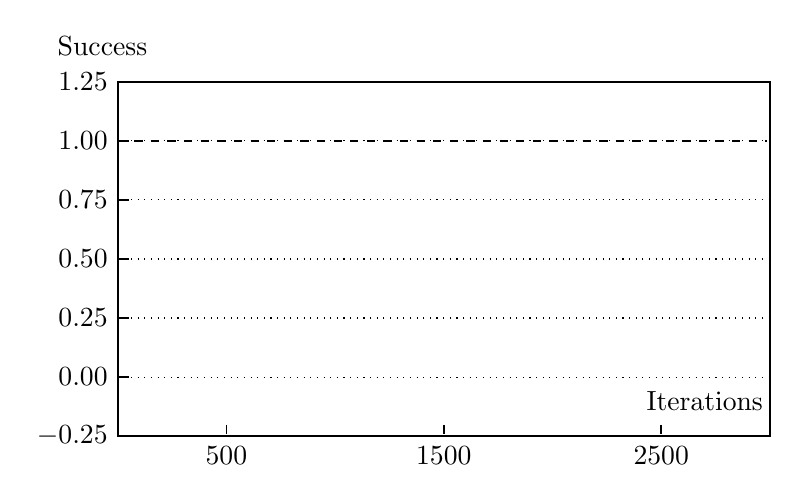
\begin{tikzpicture}[x=0.00276cm,y=3cm]
    % Draw the axes and grid lines
    \draw[-] (0,-0.25) -- (0,1.25) -- (3000,1.25) -- (3000,-0.25) -- cycle; 
    \draw[-,thin, dotted, ystep=0.25, xstep=3000] (0,-0.25) grid (3000,1.25);
    \foreach \x in {500, 1500, 2500}  \draw [-,xshift=0,yshift=-0.25](\x,-0.20) -- (\x,-0.25);
    \foreach \y in {-0.25,0.00,0.25,0.50,0.75,1.00,1.25}  \draw [-,yshift=0](4pt,\y) -- (-1pt,\y);
    \foreach \x/\xtext in {500/500, 1500/1500, 2500/2500} \node at (\x,-0.25) [below] {$\xtext$};
    \foreach \y/\ytext in {-0.25,0.00,0.25,0.50,0.75,1.00,1.25}  \node at (0,\y) [left] {$\ytext$};
    \node at (-70,1.4) {Success};
    \node at (2700,-0.1) {Iterations};
    \draw[-,red] plot[mark=x,mark size=4,mark options={color=red}] 
			file {figs/data/test05v3gmt.CP.tikzdata};
    \draw[-,blue] plot[mark=o,mark size=2,mark options={color=blue}] 
			file {figs/data/test05v3gmt.SP.tikzdata};
    % Also draw the expected convergence: 0.9^8 actions=0.43046
    \draw[dashed,-,yshift=0](0,1.0) -- (3000,1.0);

\end{tikzpicture}

   \caption{Performance of $\CLSELB$ (solid crosses) compared against $\CLSELA$ and $\BULSELA$ (both in dotted grey) in structure $\T_2$ using an applicability threshold of $0.2$.}
   \label{fig:performance-applicability}
\end{figure}


The above results show that the coverage-based confidence weighting can improve
the performance of the \CL\ approach in those cases where it performed poorly due
to false negative experiences, i.e., failure runs for a plan that includes
successful executions.
% %


Finally, we note that coverage-based selection weights encourage the agent to
explore all available options. This further ensures that all solutions are
systematically found, allowing the agent to decide which solution is optimal
faster. For some domains this may be an important feature.










%%%%%%%%%%%%%%%%%%%%%%%%%%%%%%%%%%%%%%%%%%%%%%%%%%%%


%ACKNOWLEDGMENTS are optional
%\section{Acknowledgments}
%This section is optional

%
% The following two commands are all you need in the
% initial runs of your .tex file to
% produce the bibliography for the citations in your paper.
\bibliographystyle{abbrv}
\bibliography{aamas10bdilearning}
% You must have a proper ".bib" file
%  and remember to run:
% latex bibtex latex latex
% to resolve all references
%
% ACM needs 'a single self-contained file'!
%

%APPENDICES are optional
%\balancecolumns
%\appendix
%Appendix A
%\section{Headings in Appendices}

\end{document}
